\section{留数计算}

参见《积分的方法与技巧》· 金玉明; A first course in complex analysis with applications by Dennis Zill

留数的表示
\[
\mathrm{res}_{b}f=\frac{1}{2\pi i} \oint_{C}^{} f(z) \, dz
\]
留数定理由柯西积分公式得到
\[
\oint_{C} f(z) \, \mathrm{d}z =\sum_{k=1}^{n}\oint_{C_{\epsilon}(b_k)} f(z) \, \mathrm{d}z =\sum_{k=1}^{n} 2\pi i\cdot\mathrm{res}_{b_k}f
\]
无穷远点的留数定理积分曲线方向相反 (考虑黎曼球,这是显然的)
\[
\mathrm{res}_{\infty}f=\frac{1}{2\pi i}\oint_{C^{-}} f(z) \, \mathrm{d}z=-\frac{1}{2\pi i}\oint_{C} f(z) \, \mathrm{d}z
\]
\subsection{留数的计算方法}

留数就是 $f(z)$ 的 Laurent 展开式中系数 $a_{-1}$,对于\textbf{极点}$b$,有下面较为直接的方法,不需要 Laurant 展开.

\begin{remark}
Laurant 展开就是按照公式计算
\[
\frac{1}{2\pi i} \oint_{C} f(z) \, \mathrm{d}z 
\]
\end{remark}
\subsubsection{单极点}

在 $b$ 的邻域中有
\[
f(z)=\frac{a_{-1}}{z-b}+a_0+a_1(z-b)+a_2(z-b)^2+\dots
\]
于是
\[
\mathrm{res}_{b}f=\lim_{ z \to b } (z-b)f(z)
\]
\paragraph{可表为 \texorpdfstring{$\varphi(z)/\psi(z)$}{varphi(z)/psi(z)}}

$\varphi,\psi$ 在 $b$ 点解析,且 $\varphi(b)\neq0,\psi(b)=0$,但是 $\psi'(b)\neq0$,那么
\[
\mathrm{res}_{b}f=\frac{\varphi(b)}{\psi'(b)}
\]
\subsubsection{\texorpdfstring{$n$}{n} 级极点}

Laurant 展开式为
\[
f(z)=\frac{a_{-n}}{(z-b)^{n}}+\dots+\frac{a_{-1}}{z-b}+a_0+a_1(z-b)+\dots
\]
那么
\[
(z-b)^{n}f(z)=a_{-n}+a_{-n+1}(z-b)+\dots+a_{-1}(z-b)^{n-1}+a_0(z-b)^{n}+\dots
\]
两边 $\frac{\mathrm{d}^{n-1}}{\mathrm{d}z^{n-1}}$ 得到
\[
\lim_{ z \to b } \frac{\mathrm{d}^{n-1}}{\mathrm{d}z^{n-1}} [(z-b)^{n}f(z)]=(n-1)!a_{-1}
\]
于是
\[
\mathrm{res}_{b}f=\frac{1}{(n-1)!}\cdot \lim_{ z \to b } \frac{\mathrm{d}^{n-1}}{\mathrm{d}z^{n-1}} [(z-b)^{n}f(z)]
\]
\subsection{计算定积分}

详细计算见《积分的方法与技巧》· 金玉明 p 328

\label{jflajlf}

\subsubsection{Jordan 引理}

\begin{lemma}[Jordan's Lemma]
Let $C_R$ be a semicircular contour in the upper half-plane defined by $z = Re^{i\theta}$ for $0 \leq \theta \leq \pi$. Suppose $f(z)$ is a function that is analytic in the upper half-plane for $|z| > R_0$ (for some constant $R_0$).
If $f(z) \to 0$ uniformly as $|z| \to \infty$ for $z$ in the upper half-plane (i.e., $M_R = \max_{z \in C_R} |f(z)| \to 0$ as $R \to \infty$), then for any real constant $m > 0$,
\[
\lim_{R \to \infty} \int_{C_R} f(z)e^{imz} dz = 0
\]
A similar statement holds for a semicircular contour in the lower half-plane if $m < 0$.\label{3910a9}
\end{lemma}

\begin{proof}
Let $m>0$, denote
\[
I_{R}\coloneqq \int_{0}^{\pi} f(R e^{ i\theta })e^{ im(Re^{ i\theta }) }(i R e^{ i\theta }) \, \mathrm{d}\theta 
\]
Estmate the value,
\[
\begin{aligned}
\lvert I_{R} \rvert  & =\left\lvert  \int_{0}^{\pi} f(R e^{ i\theta })e^{ im(Re^{ i\theta }) }(i R e^{ i\theta }) \, \mathrm{d}\theta   \right\rvert  \\
 & \leq \int_{0}^{\pi} \underbrace{ \lvert f(R e^{ i\theta }) \rvert }_{ \leq M_{R} } \cdot \underbrace{ \lvert e^{ im(Re^{ i\theta }) } \rvert }_{ =\exp \{ -mR\sin\theta \} } \cdot \underbrace{ \lvert iR e^{ i\theta } \rvert }_{ =R }    \, \mathrm{d}\theta \\
 & \leq 2RM_{R}\int_{0}^{\pi/2 } e^{ -mR\sin\theta } \, \mathrm{d}\theta \\
 & \overset{ \sin\theta\geq  \frac{2}{\pi}\theta }{ \leq  }2RM_{R}\underbrace{ \int_{0}^{\pi/2 } e^{ -\frac{2}{\pi}mR\theta } \, \mathrm{d}\theta  }_{ =\frac{1}{\frac{2}{\pi}mR}(1-e^{ -mR }) } \\
 & =\frac{\pi M_{R}(1-e^{ -mR })}{m}\to0\qquad \text{as }R\to \infty
\end{aligned}
\]
\end{proof}

\section{围道积分}

参见 A first course in complex analysis with applications by Dennis Zill, Section 6.6

\subsection{Basic Integrations}

Given the integrals of the form
\begin{equation}
\int_{0}^{2\pi} F(\cos\theta,\sin\theta) \, \mathrm{d}\theta
\label{09155c}
\end{equation}

To convert it to a complex integral on $\lvert z \rvert=1$, we parametrize the contour by $z=e^{ i\theta },0\leq\theta\leq2\pi$. We can then write
\[
dz=ie^{ i\theta }d\theta,\quad \cos\theta=\frac{e^{ i\theta }+e^{ -i\theta }}{2},\quad \sin\theta=\frac{e^{ i\theta }-e^{ -i\theta }}{2i}
\]
i.e.
\[
d\theta=\frac{dz}{iz},\quad\cos\theta=\frac{1}{2}(z+z^{-1}),\quad\sin\theta=\frac{1}{2i}(z-z^{-1}).
\]
Then \cref{09155c} becomes
\[
\oint_{C}F\left( \frac{1}{2}(z+z^{-1}),\frac{1}{2i}(z-z^{-1}) \right)\,\frac{dz }{iz}
\]
where $C$ is the unit circle $\lvert z \rvert=1$.

\begin{figure}[H]
\centering
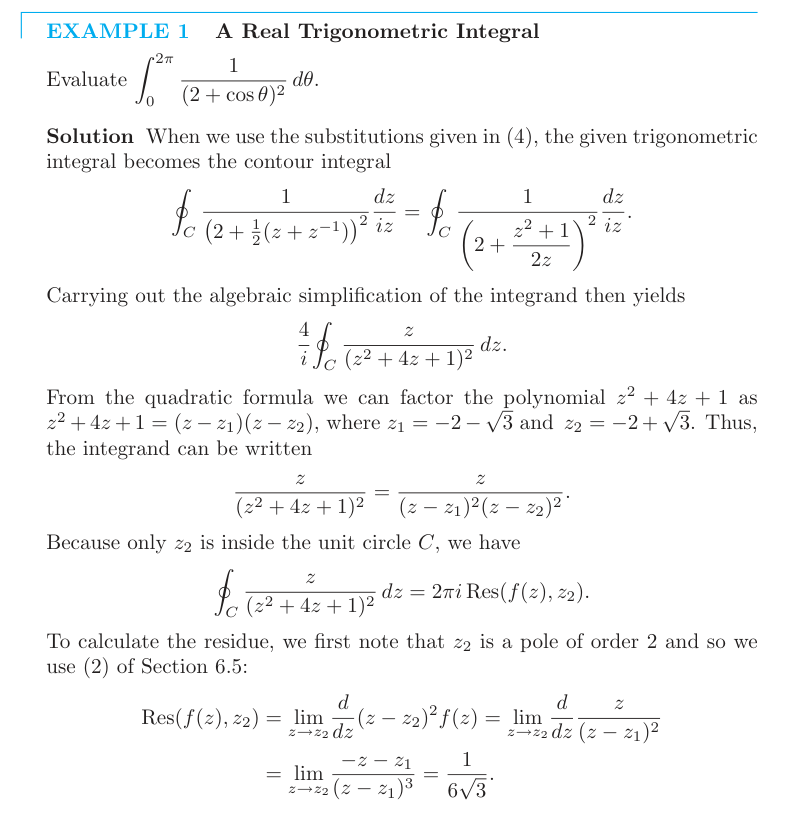
\includegraphics[width=\textwidth]{留数计算方法-2025051500.png}
% \caption{}
\label{}
\end{figure}
\begin{figure}[H]
\centering
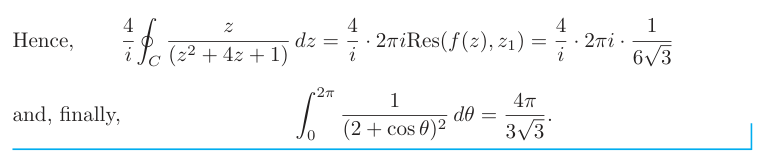
\includegraphics[width=\textwidth]{1-留数计算方法-2025051500.png}
% \caption{}
\label{}
\end{figure}

Cauchy principal value of an integral is defined by
\[
\mathrm{P.V.}\int_{-\infty}^{\infty}f(x)dx=\lim_{R\to\infty}\int_{-R}^{R}f(x)dx.
\]
If a integral diverges, it may still possess a Cauchy principal value.

\begin{figure}[H]
\centering
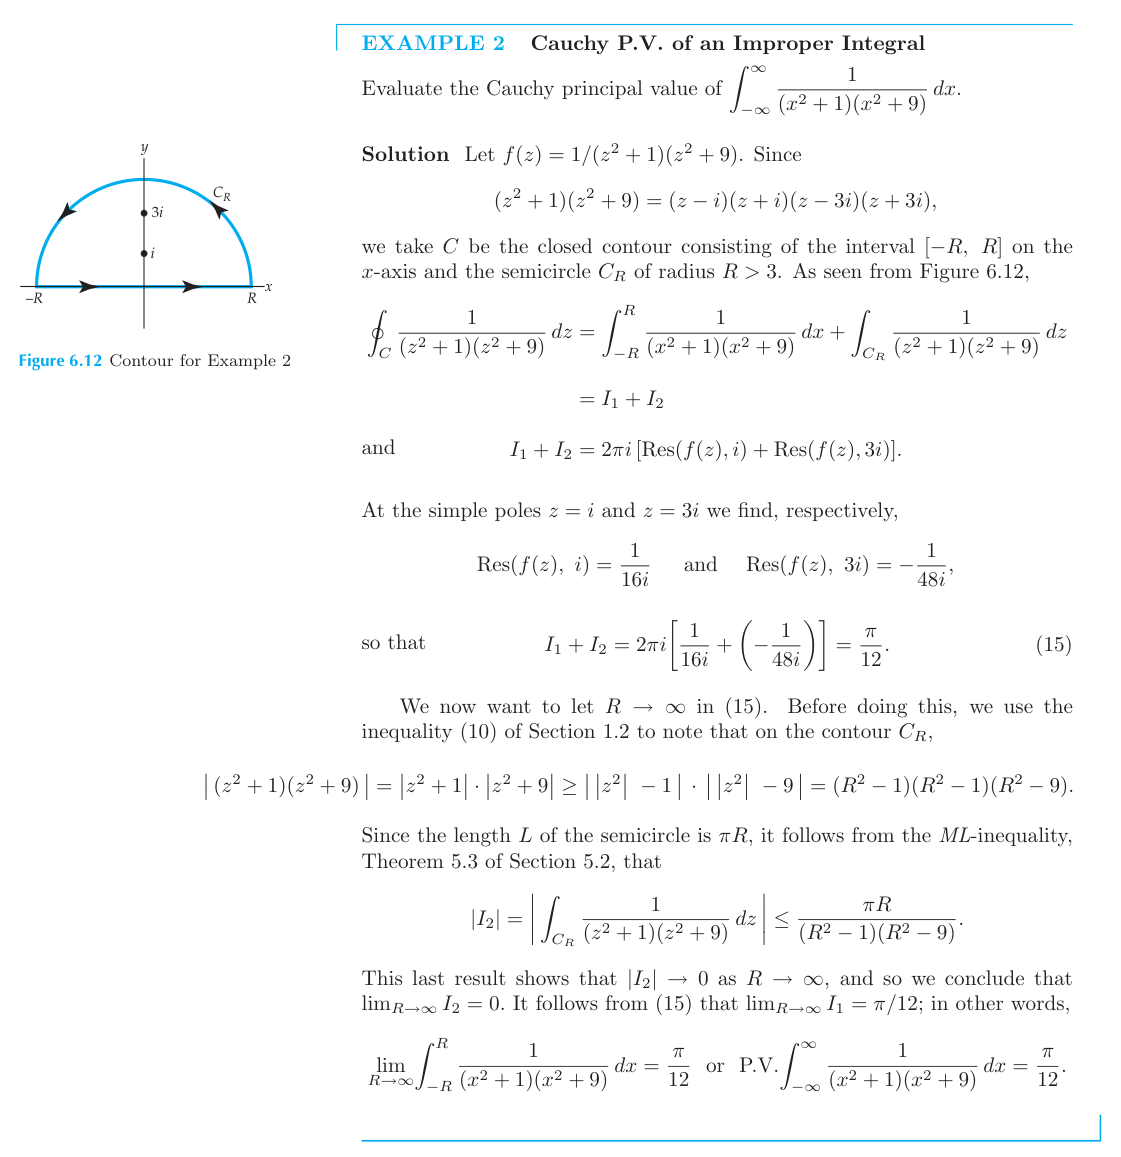
\includegraphics[width=\textwidth]{2-留数计算方法-2025051500.png}
% \caption{}
\label{}
\end{figure}

\begin{figure}[H]
\centering
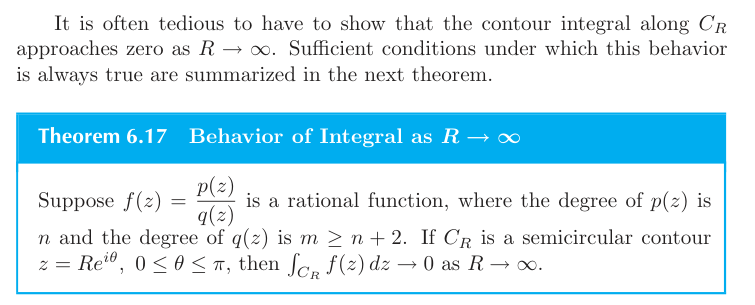
\includegraphics[width=\textwidth]{3-留数计算方法-2025051500.png}
% \caption{}
\label{}
\end{figure}

Another powerful lemma is \cref{3910a9}.

Next we calculate
\[
\int_{-\infty}^{\infty} F(x)\sin\alpha x \, \mathrm{d}x ,\qquad \int_{-\infty}^{\infty} F(x)\cos\alpha x\, \mathrm{d}x 
\]
\begin{figure}[H]
\centering
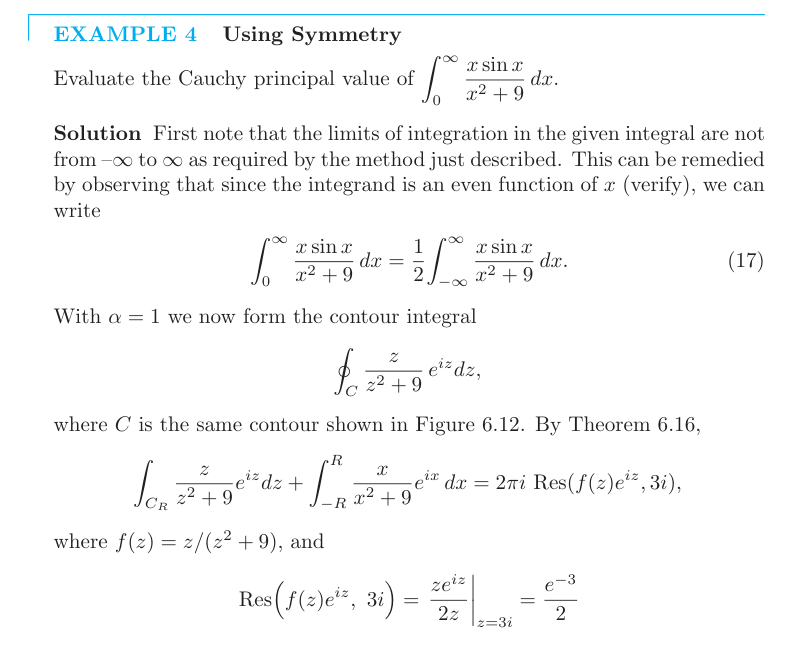
\includegraphics[width=\textwidth]{4-留数计算方法-2025051500.png}
% \caption{}
\label{}
\end{figure}
\begin{figure}[H]
\centering
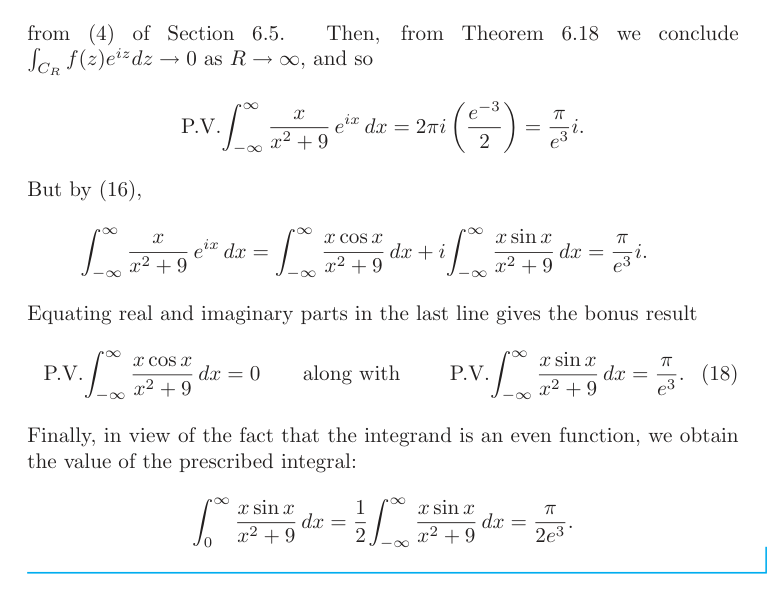
\includegraphics[width=\textwidth]{5-留数计算方法-2025051500.png}
% \caption{}
\label{}
\end{figure}

Indented contour is of great use.

\begin{figure}[H]
\centering
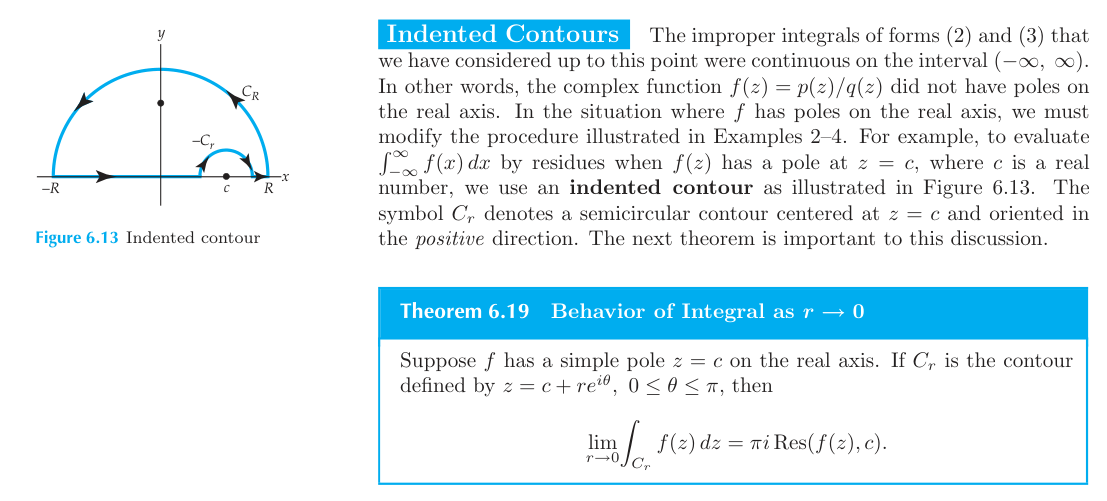
\includegraphics[width=\textwidth]{6-留数计算方法-2025051500.png}
% \caption{}
\label{}
\end{figure}

\begin{figure}[H]
\centering
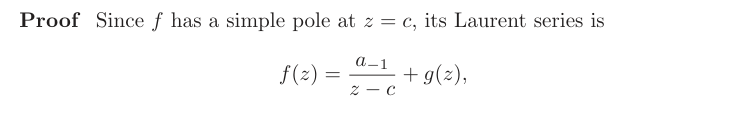
\includegraphics[width=\textwidth]{7-留数计算方法-2025051500.png}
% \caption{}
\label{}
\end{figure}

\begin{figure}[H]
\centering
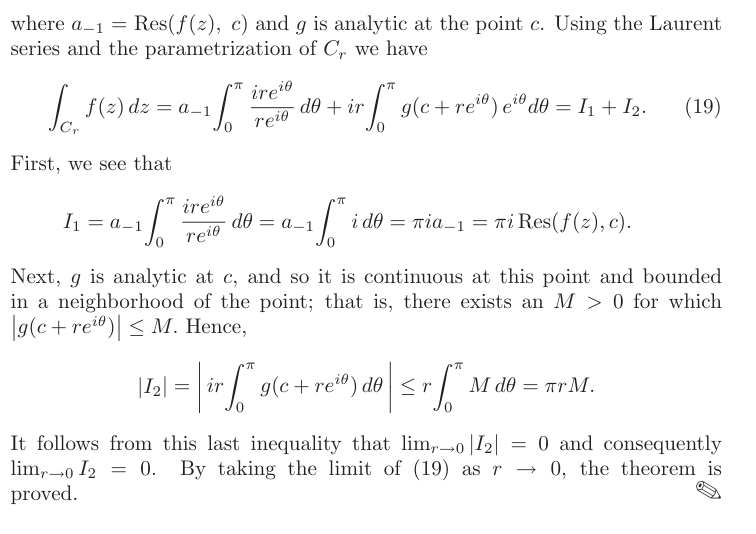
\includegraphics[width=\textwidth]{8-留数计算方法-2025051500.png}
% \caption{}
\label{}
\end{figure}

\begin{figure}[H]
\centering
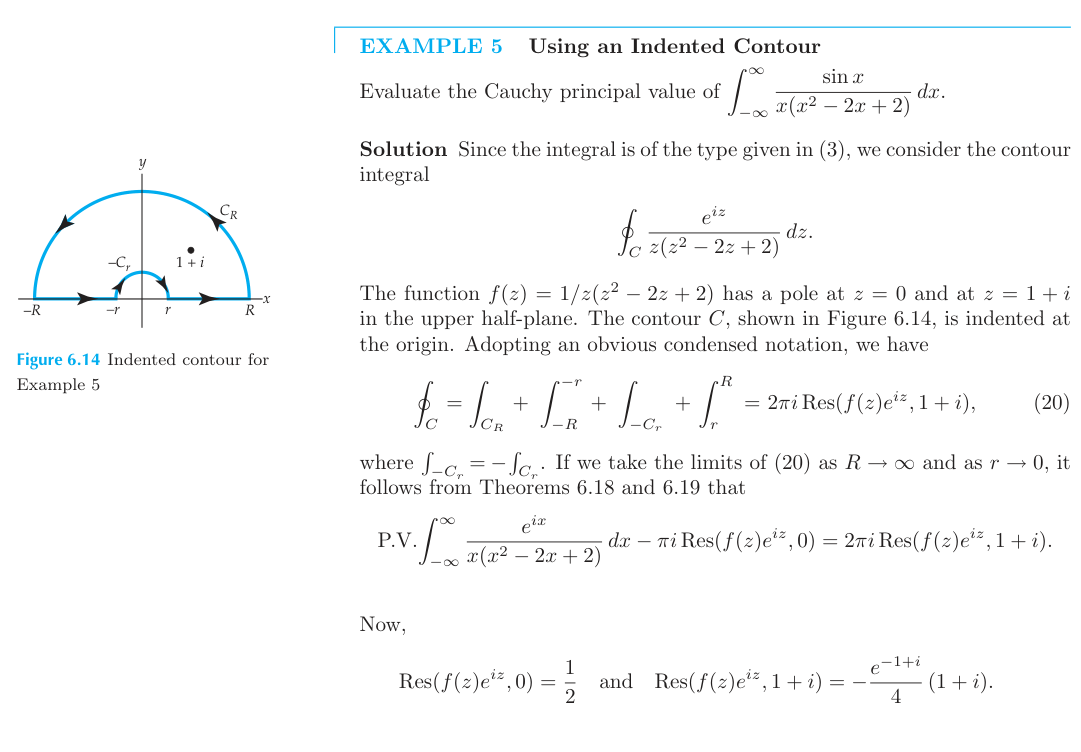
\includegraphics[width=\textwidth]{9-留数计算方法-2025051500.png}
% \caption{}
\label{}
\end{figure}
\begin{figure}[H]
\centering
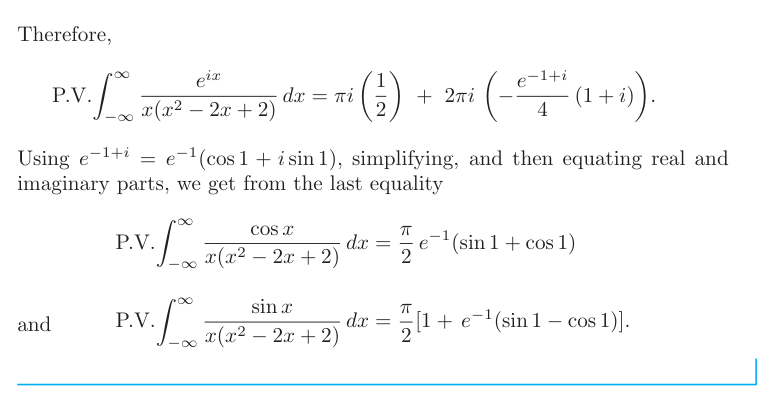
\includegraphics[width=\textwidth]{10-留数计算方法-2025051500.png}
% \caption{}
\label{}
\end{figure}

\subsection{Integration along a Branch cut}

In the next discussion we examine integration along a Branch cut (cf section 2.6 and 4.1 in Dennis Zill)

\begin{figure}[H]
\centering
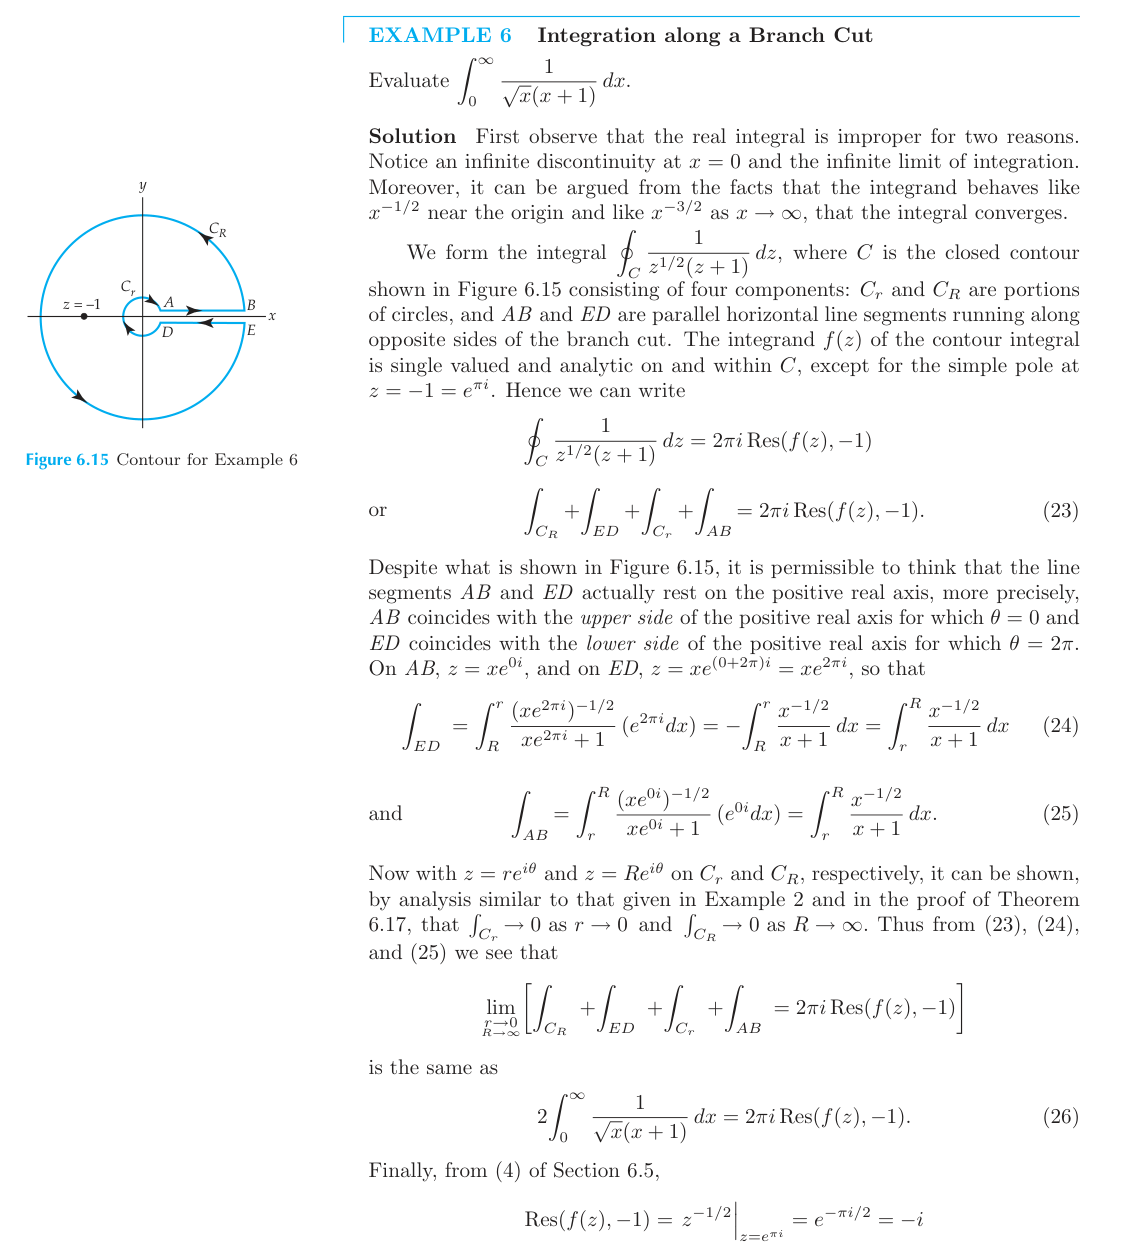
\includegraphics[width=\textwidth]{11-留数计算方法-2025051500.png}
% \caption{}
\label{}
\end{figure}
\begin{figure}[H]
\centering
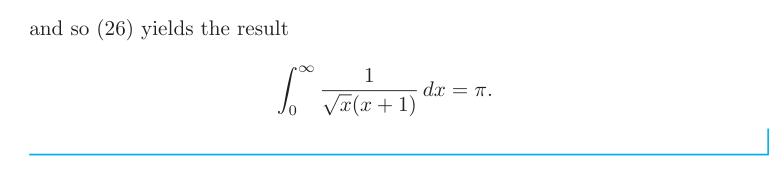
\includegraphics[width=\textwidth]{12-留数计算方法-2025051500.png}
% \caption{}
\label{}
\end{figure}

This technique also goes for $\mathrm{Ln}z$.

\subsection{The Argument Principle and Rouche's Theorem}

\subsubsection{Argument Principle}

\begin{figure}[H]
\centering
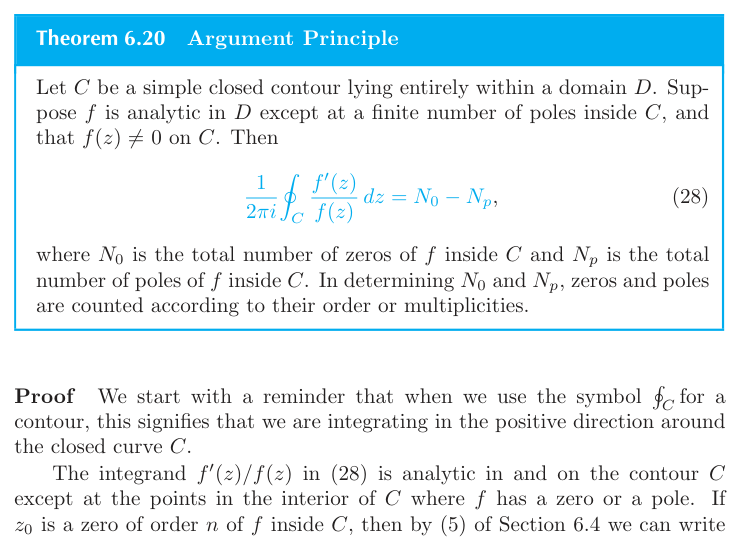
\includegraphics[width=\textwidth]{13-留数计算方法-2025051500.png}
% \caption{}
\label{}
\end{figure}
\begin{figure}[H]
\centering
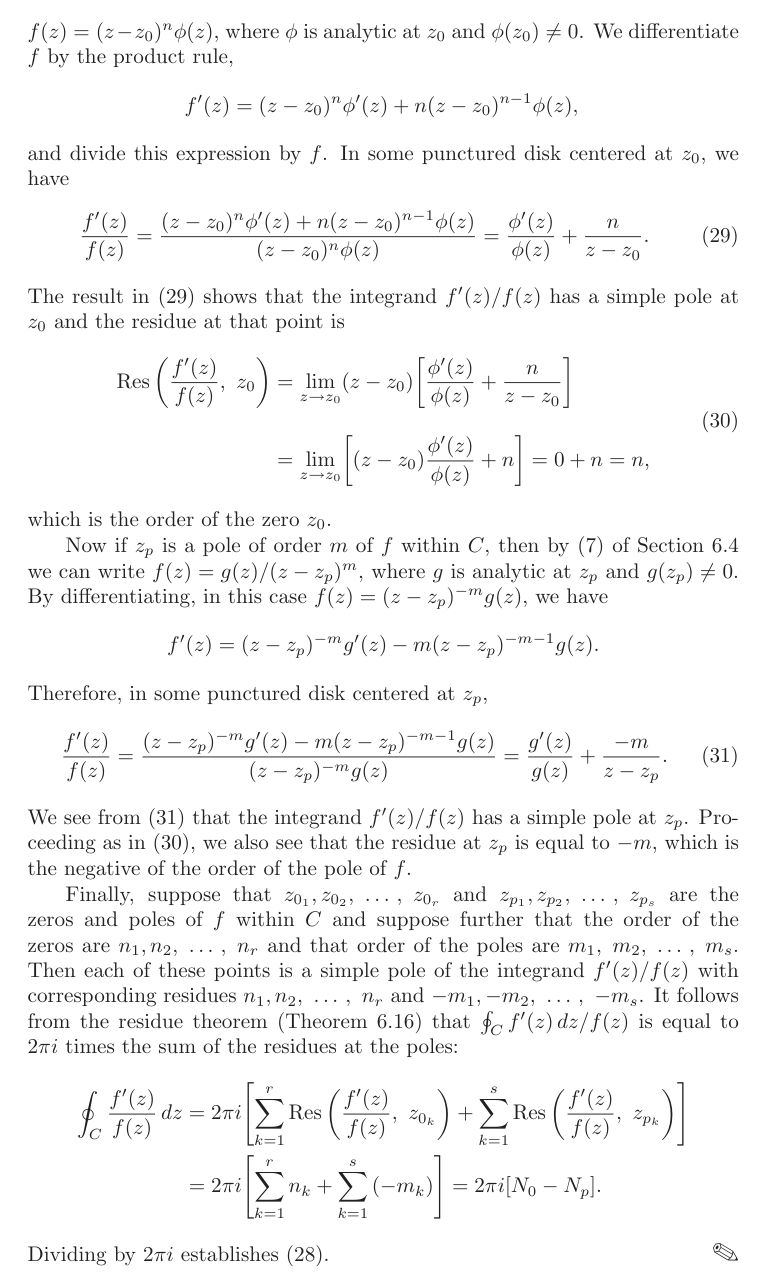
\includegraphics[width=\textwidth]{14-留数计算方法-2025051500.png}
% \caption{}
\label{}
\end{figure}

\paragraph{Why the name?}

\begin{figure}[H]
\centering
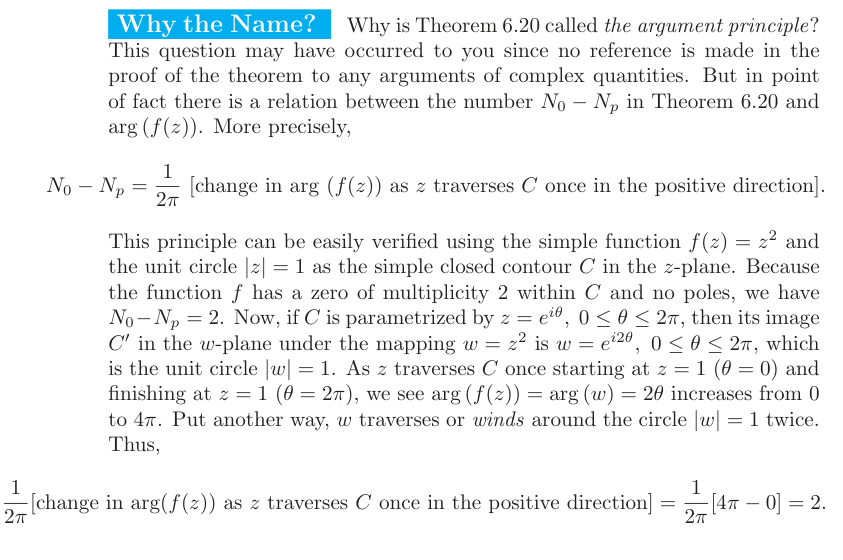
\includegraphics[width=\textwidth]{15-留数计算方法-2025051500.png}
% \caption{}
\label{}
\end{figure}

\subsubsection{Rouche's theorem}

Rouche's theorem is a consequence of Argument Principle.

\begin{figure}[H]
\centering
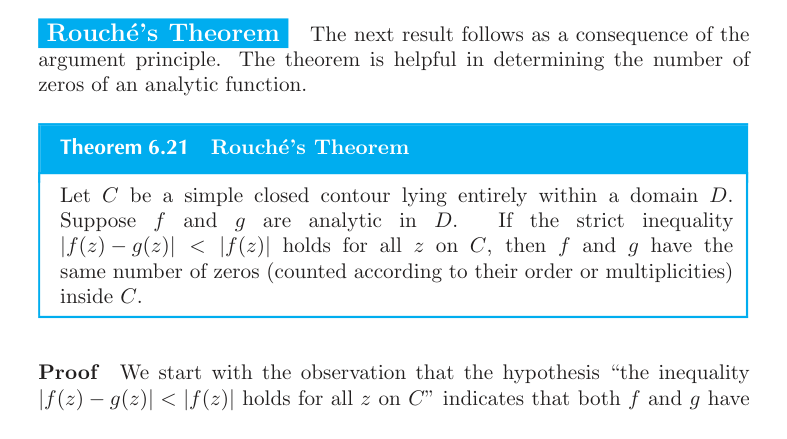
\includegraphics[width=\textwidth]{17-留数计算方法-2025051500.png}
% \caption{}
\label{}
\end{figure}
\begin{figure}[H]
\centering
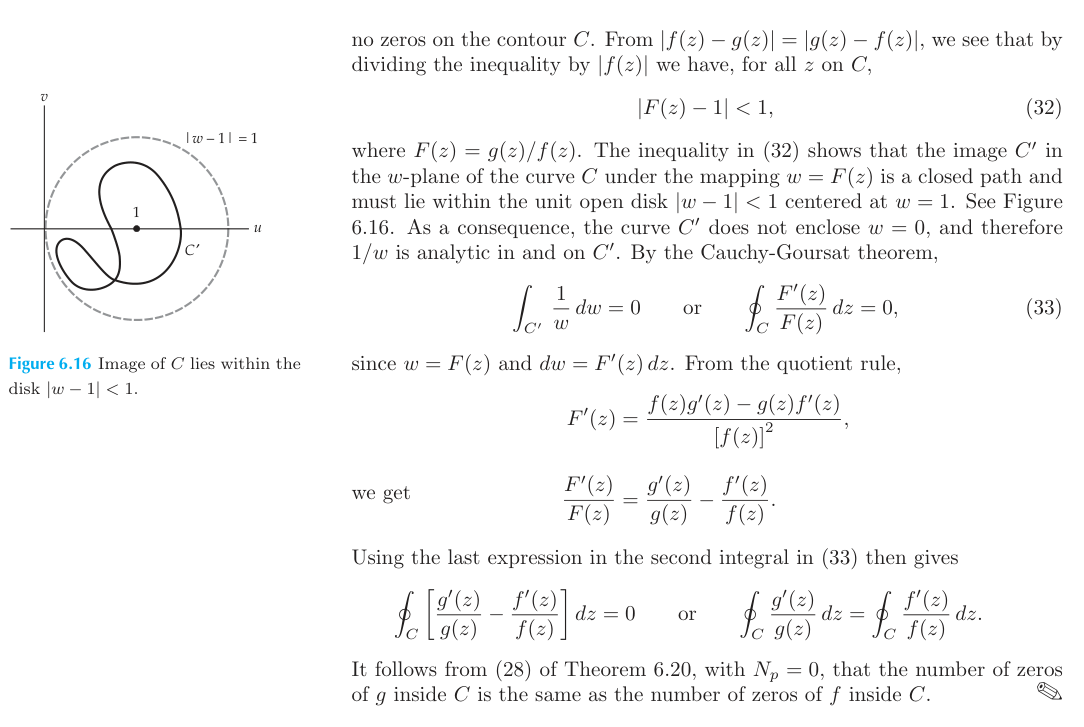
\includegraphics[width=\textwidth]{18-留数计算方法-2025051500.png}
% \caption{}
\label{}
\end{figure}

\subsection{Summing Infinite Series}

\begin{figure}[H]
\centering
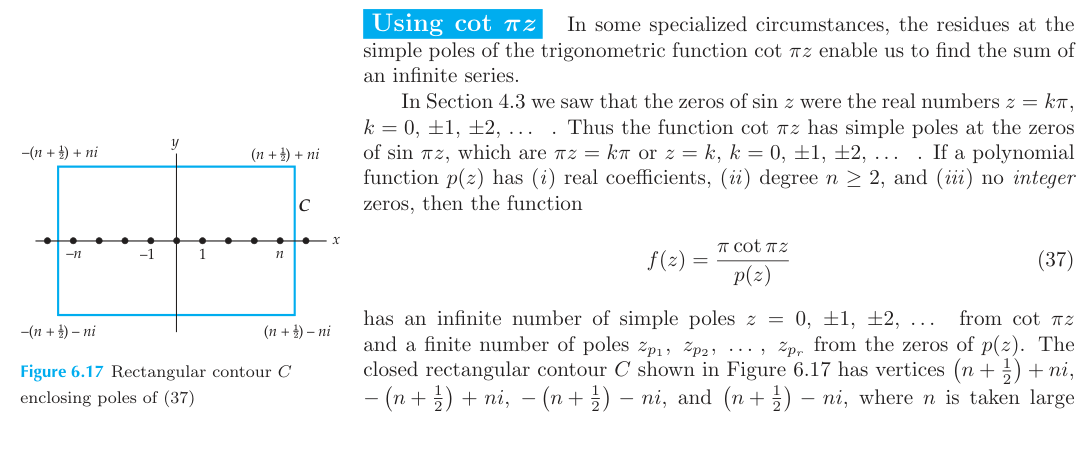
\includegraphics[width=\textwidth]{19-留数计算方法-2025051500.png}
% \caption{}
\label{}
\end{figure}
\begin{figure}[H]
\centering
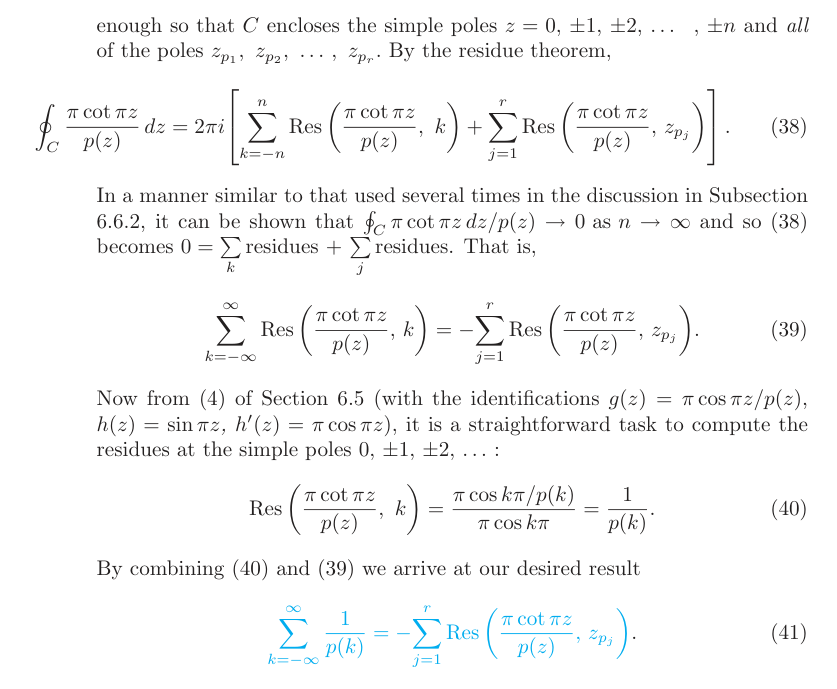
\includegraphics[width=\textwidth]{20-留数计算方法-2025051500.png}
% \caption{}
\label{}
\end{figure}

\begin{figure}[H]
\centering
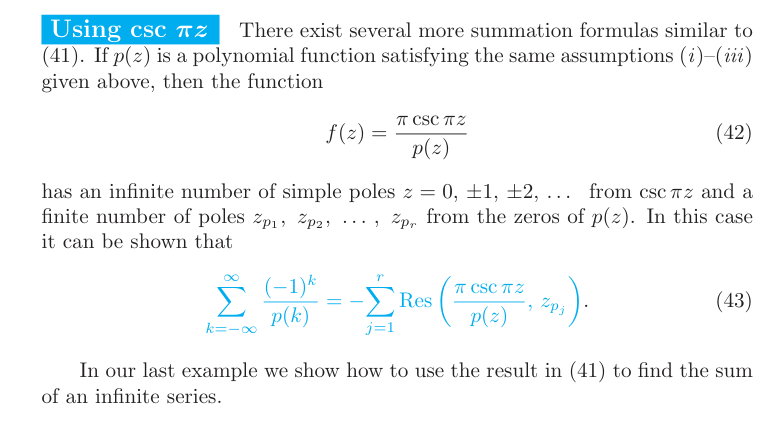
\includegraphics[width=\textwidth]{21-留数计算方法-2025051500.png}
% \caption{}
\label{}
\end{figure}

\begin{figure}[H]
\centering
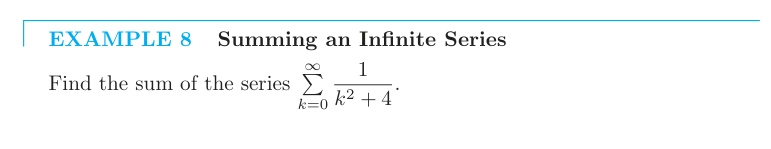
\includegraphics[width=\textwidth]{22-留数计算方法-2025051500.png}
% \caption{}
\label{}
\end{figure}

\begin{figure}[H]
\centering
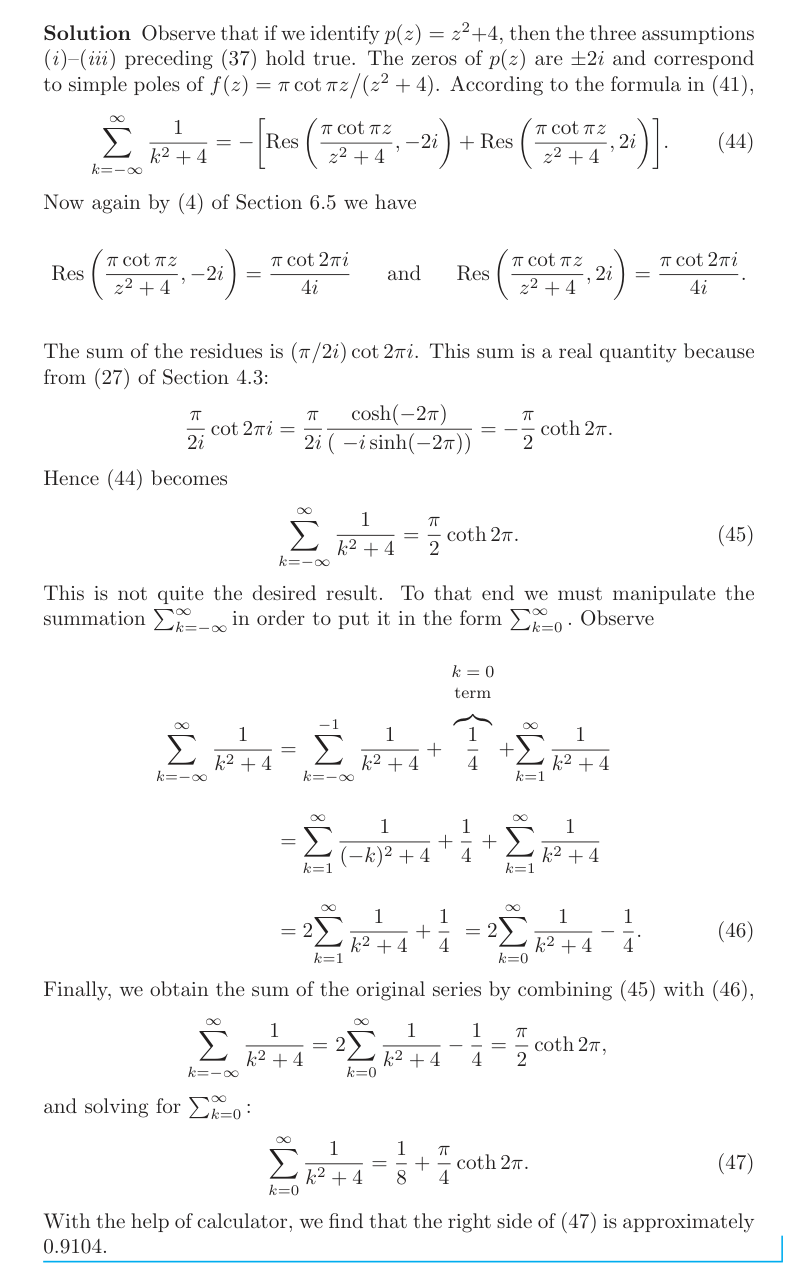
\includegraphics[width=\textwidth]{23-留数计算方法-2025051500.png}
% \caption{}
\label{}
\end{figure}

\section{Complex Integration (Ph. D qualifying test)}

\subsection{单值性}

\begin{figure}[H]
\centering
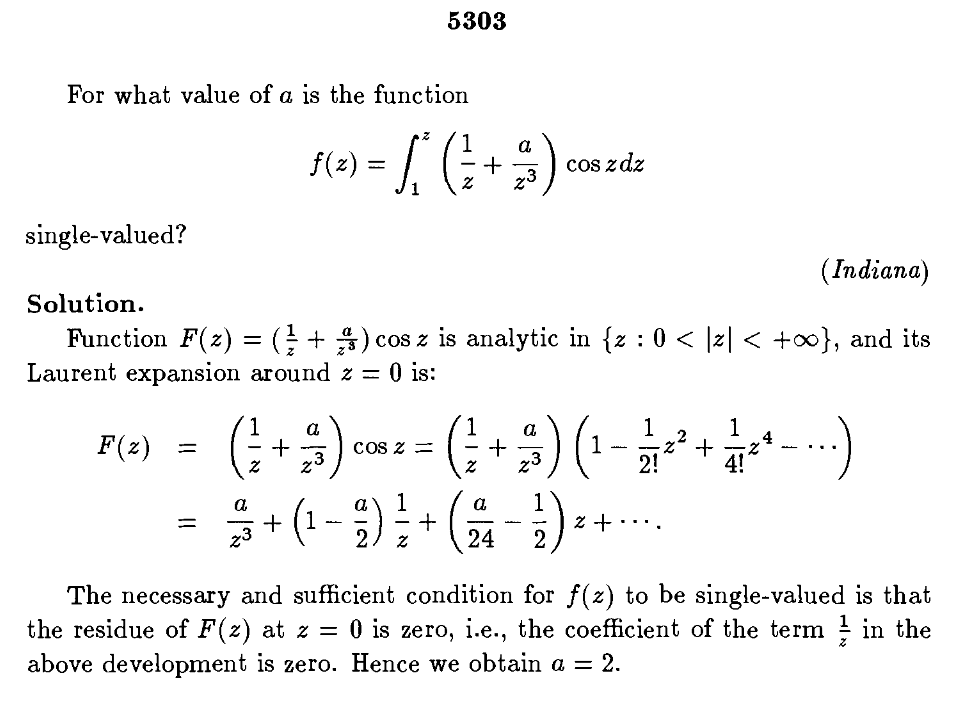
\includegraphics[width=\textwidth]{留数计算方法-2025061023.png}
% \caption{}
\label{}
\end{figure}

\subsection{积分恒等式}

\begin{figure}[H]
\centering
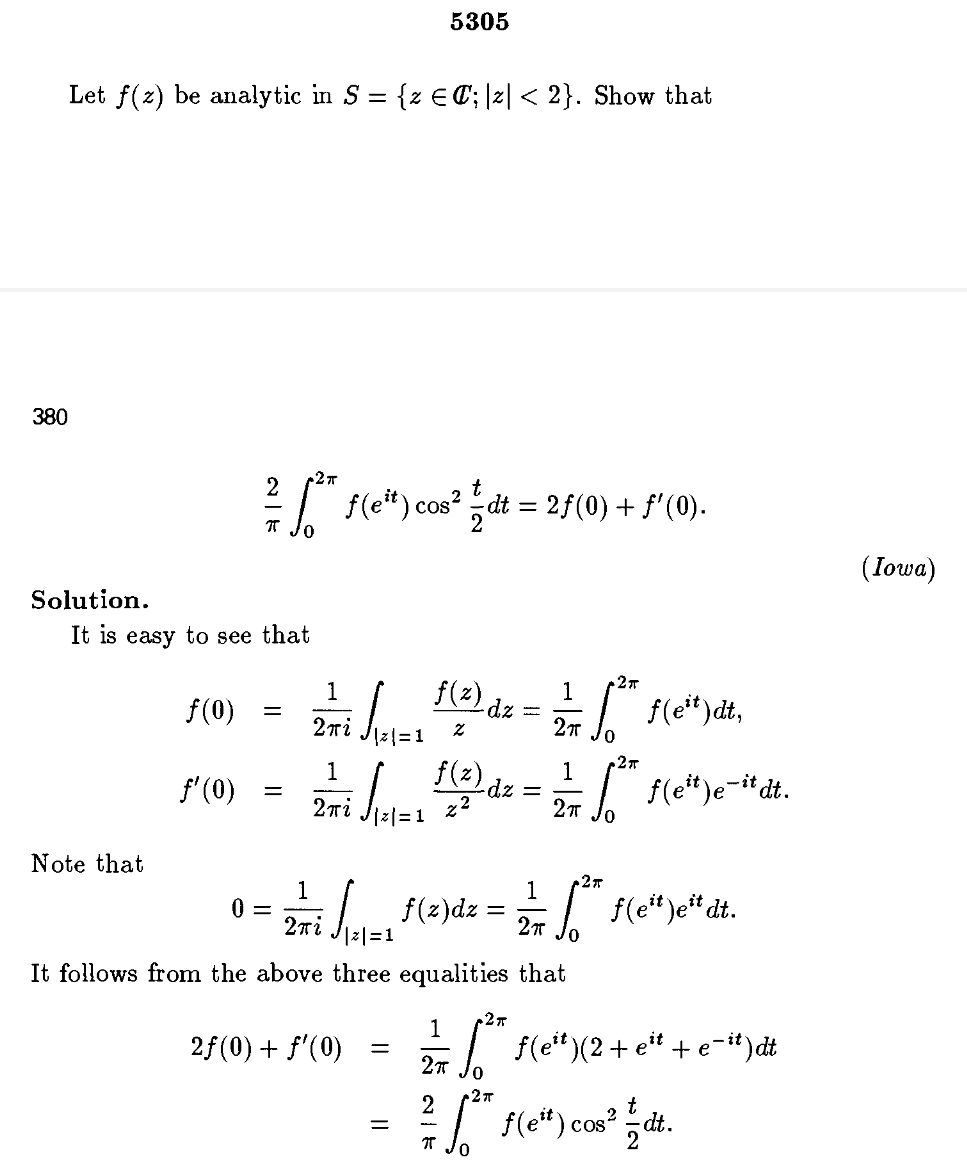
\includegraphics[width=\textwidth]{留数计算方法-2025061100.png}
% \caption{}
\label{}
\end{figure}

\subsection{有关实部和虚部的积分不等式}

\begin{figure}[H]
\centering
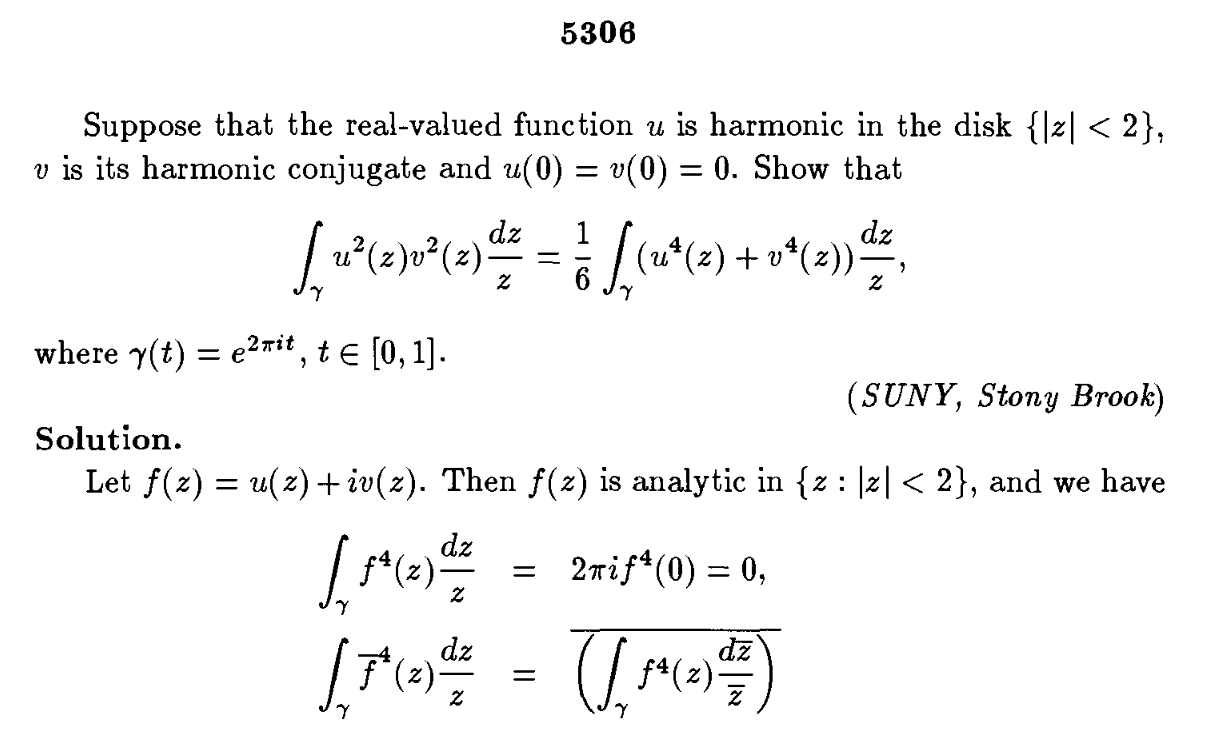
\includegraphics[width=\textwidth]{留数计算方法-2025061110.png}
% \caption{}
\label{}
\end{figure}
\begin{figure}[H]
\centering
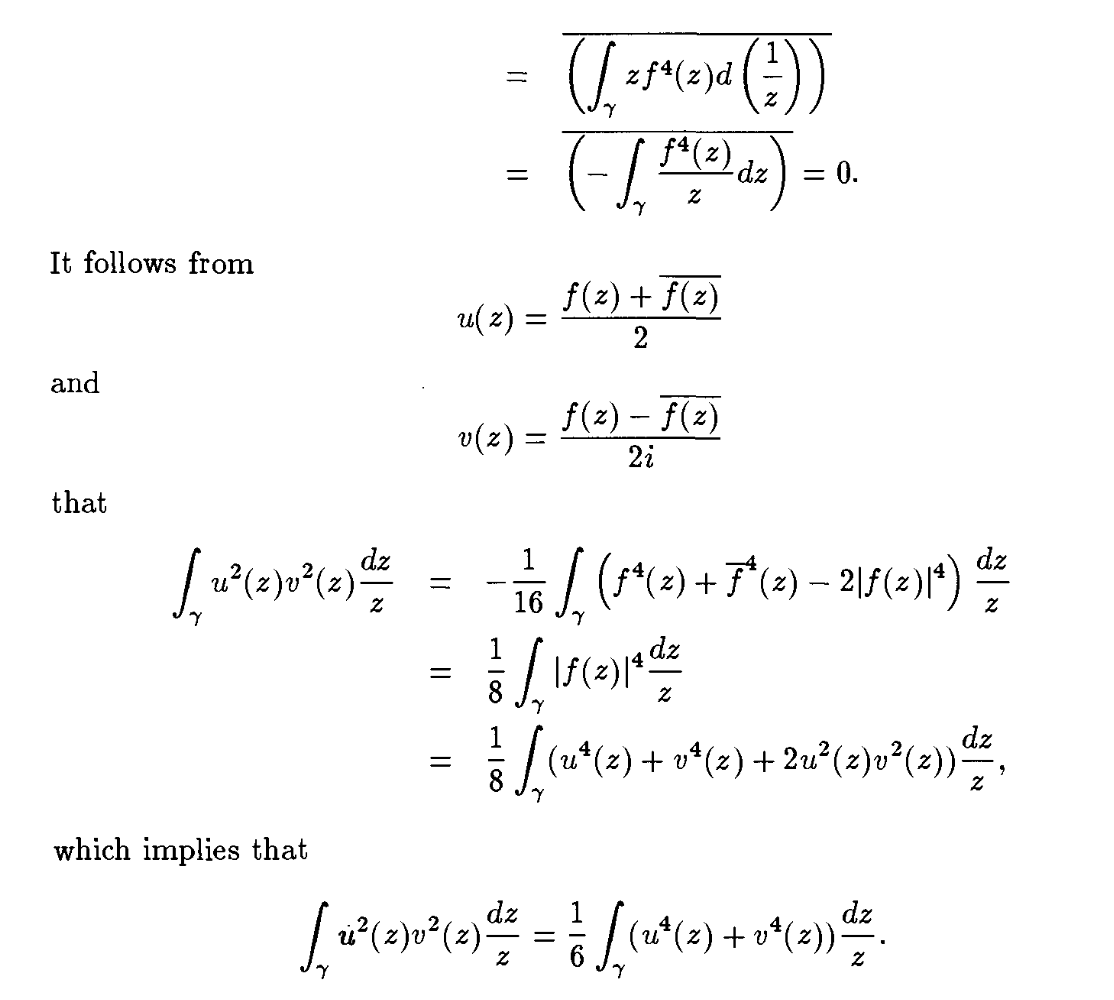
\includegraphics[width=\textwidth]{1-留数计算方法-2025061110.png}
% \caption{}
\label{}
\end{figure}

\subsection{关于 \texorpdfstring{$\text{Re }f$}{textRe f} 的积分恒等式}

\begin{figure}[H]
\centering
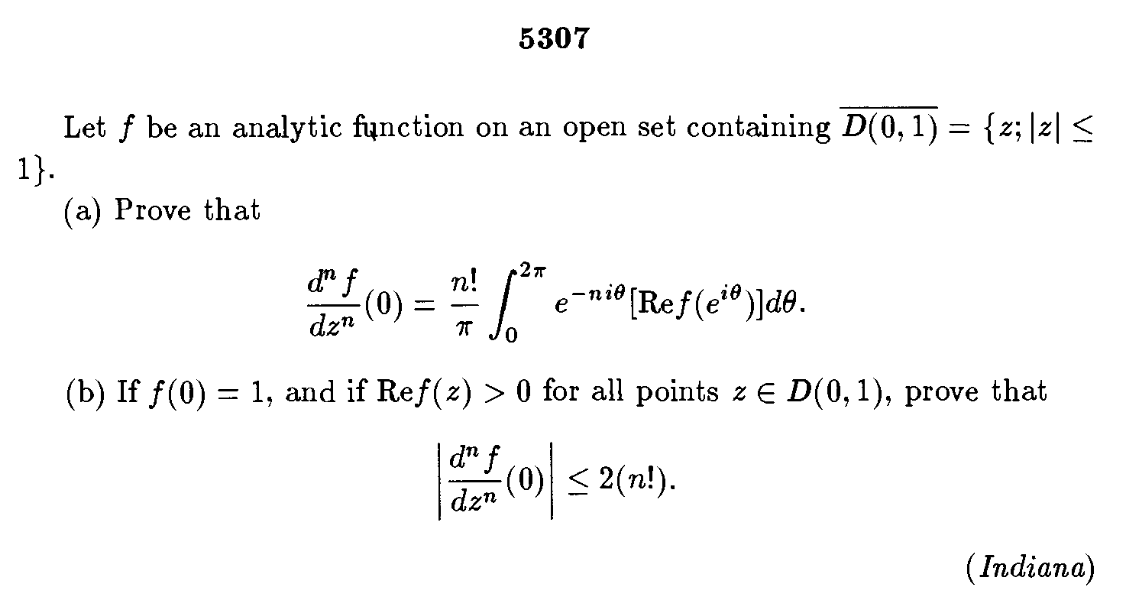
\includegraphics[width=\textwidth]{2-留数计算方法-2025061110.png}
% \caption{}
\label{}
\end{figure}
\begin{figure}[H]
\centering
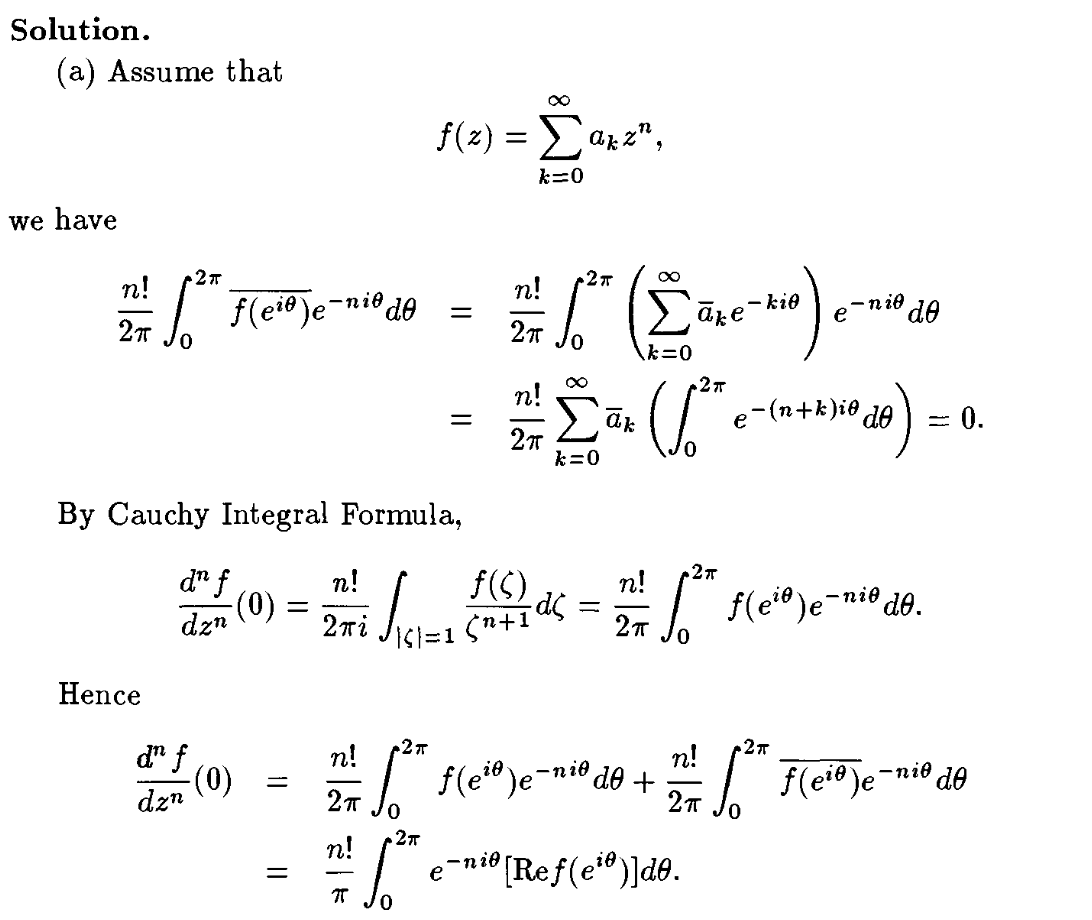
\includegraphics[width=\textwidth]{3-留数计算方法-2025061110.png}
% \caption{}
\label{}
\end{figure}
\begin{figure}[H]
\centering
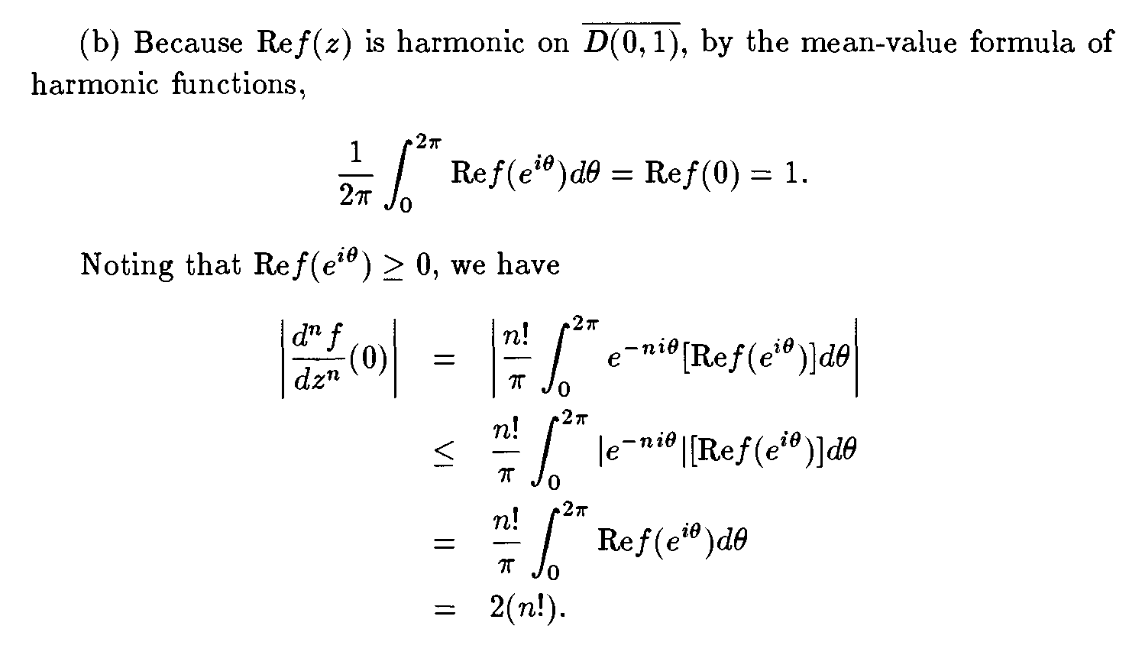
\includegraphics[width=\textwidth]{5-留数计算方法-2025061110.png}
% \caption{}
\label{}
\end{figure}

\subsection{应用 Cauchy 积分公式}

\begin{figure}[H]
\centering
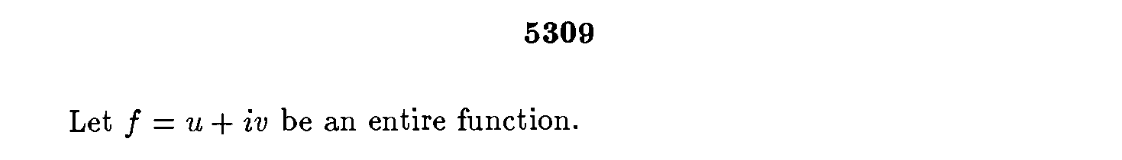
\includegraphics[width=\textwidth]{6-留数计算方法-2025061110.png}
% \caption{}
\label{}
\end{figure}
\begin{figure}[H]
\centering
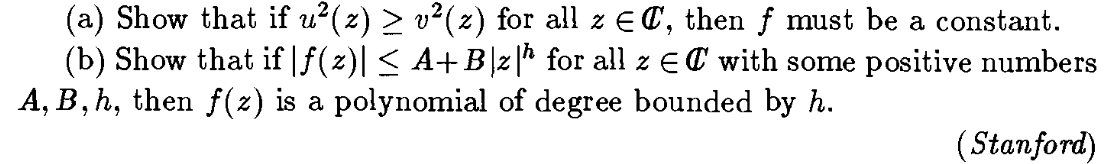
\includegraphics[width=\textwidth]{7-留数计算方法-2025061110.png}
% \caption{}
\label{}
\end{figure}
\begin{figure}[H]
\centering
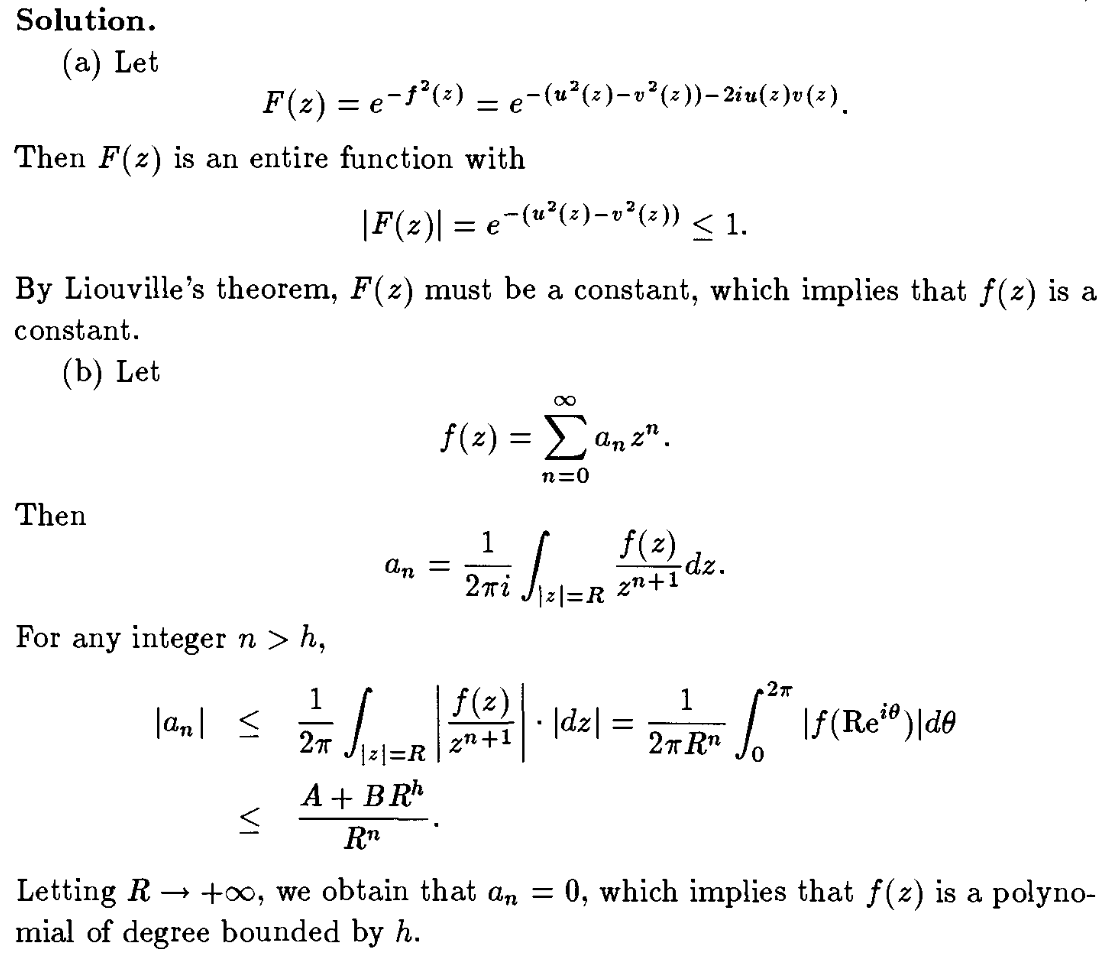
\includegraphics[width=\textwidth]{8-留数计算方法-2025061110.png}
% \caption{}
\label{}
\end{figure}

\subsection{复形式 Green 公式}

\begin{figure}[H]
\centering
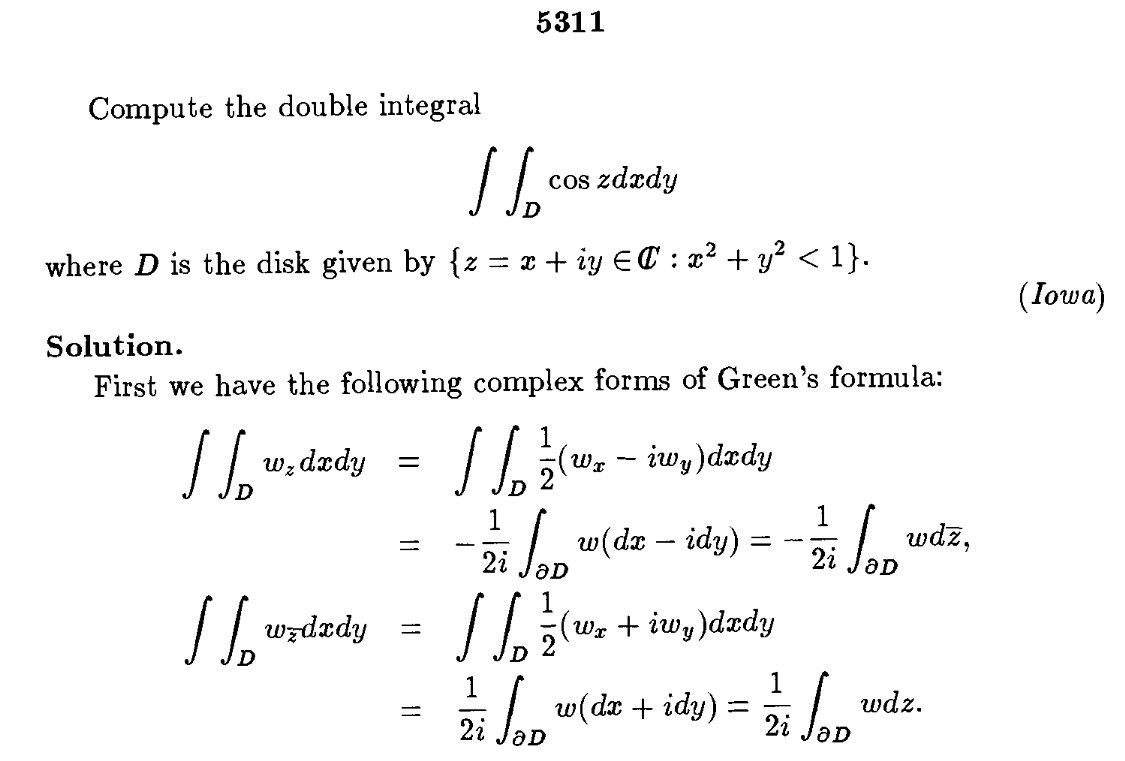
\includegraphics[width=\textwidth]{9-留数计算方法-2025061110.png}
% \caption{}
\label{}
\end{figure}
\begin{figure}[H]
\centering
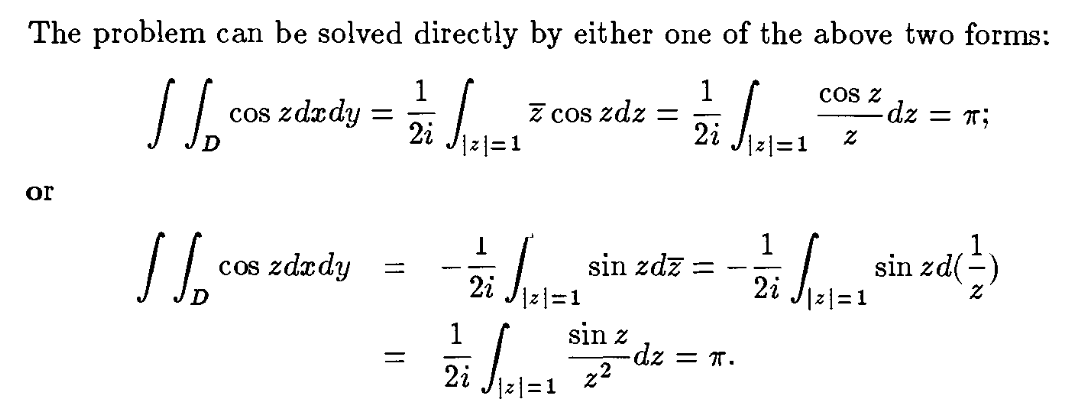
\includegraphics[width=\textwidth]{10-留数计算方法-2025061110.png}
% \caption{}
\label{}
\end{figure}

\begin{note}
这里利用到 $\frac{ \partial   }{ \partial \overline{z} }\overline{z}\cos z=\cos z$. $\partial_{\overline{z}}$ 并不会影响到 $f(z)$.
\end{note}
\subsection{面积公式}

\begin{figure}[H]
\centering
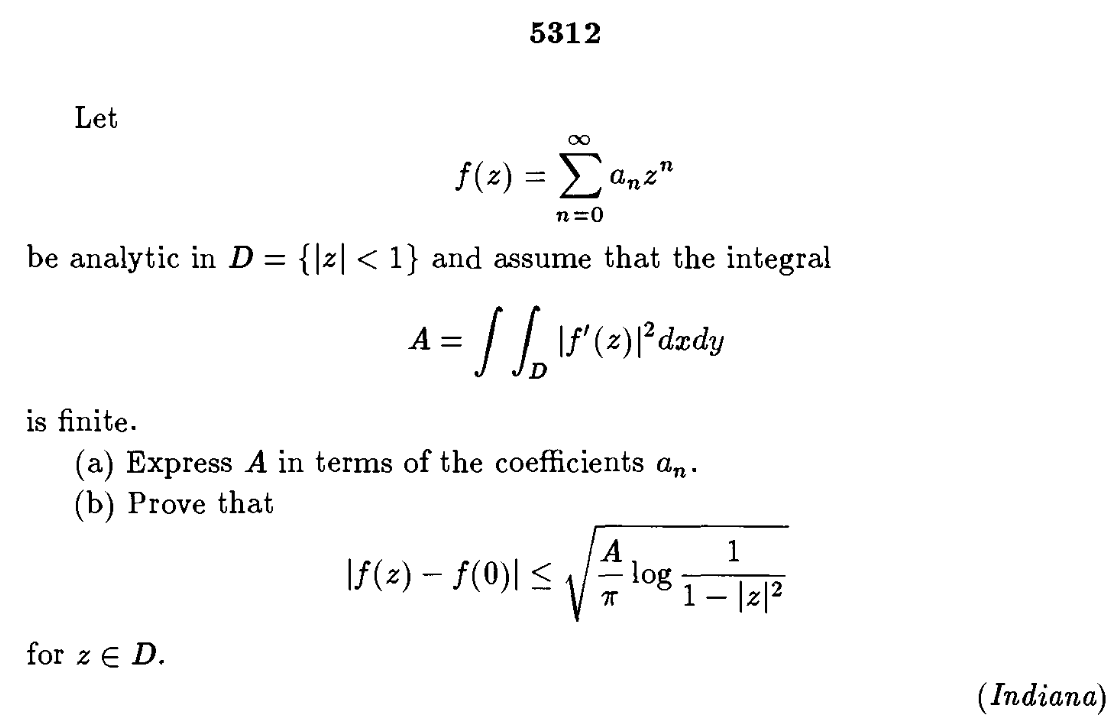
\includegraphics[width=\textwidth]{留数计算方法-2025061111.png}
% \caption{}
\label{}
\end{figure}

\begin{figure}[H]
\centering
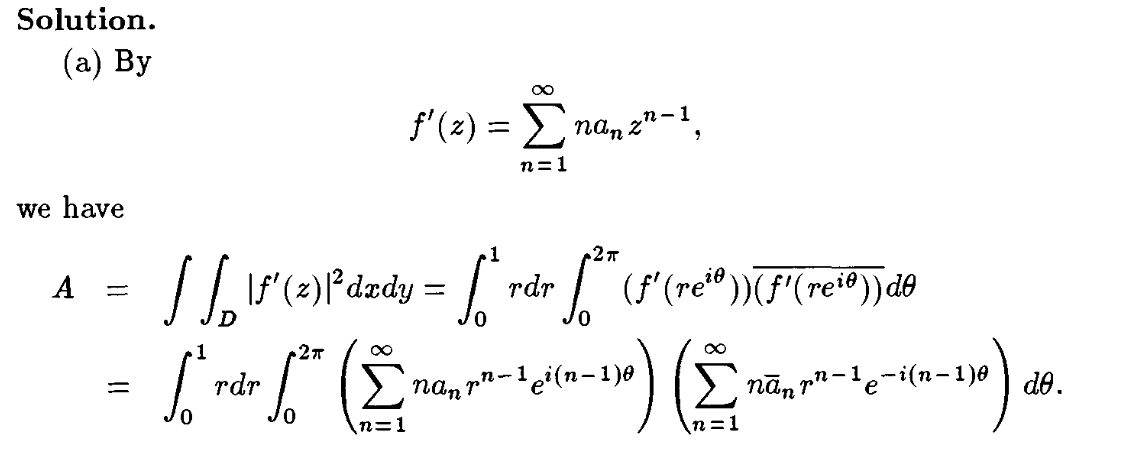
\includegraphics[width=\textwidth]{1-留数计算方法-2025061111.png}
% \caption{}
\label{}
\end{figure}

\begin{figure}[H]
\centering
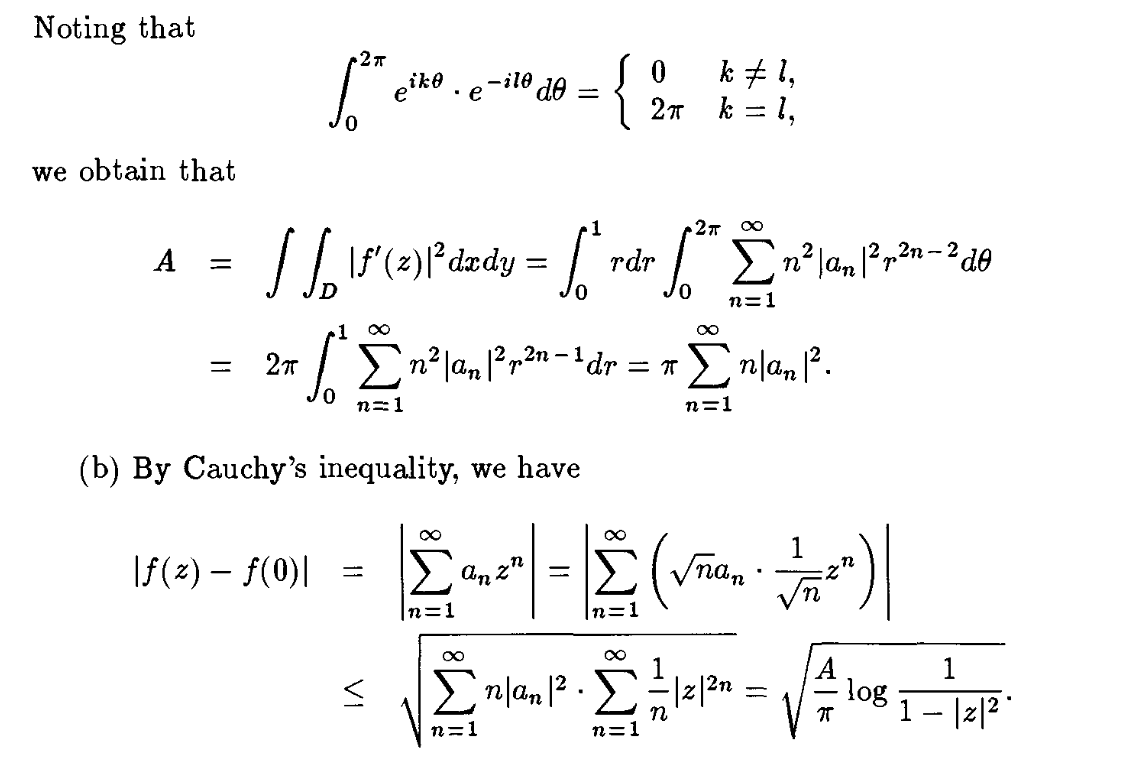
\includegraphics[width=\textwidth]{2-留数计算方法-2025061111.png}
% \caption{}
\label{}
\end{figure}

\subsection{应用留数定理}

\begin{figure}[H]
\centering
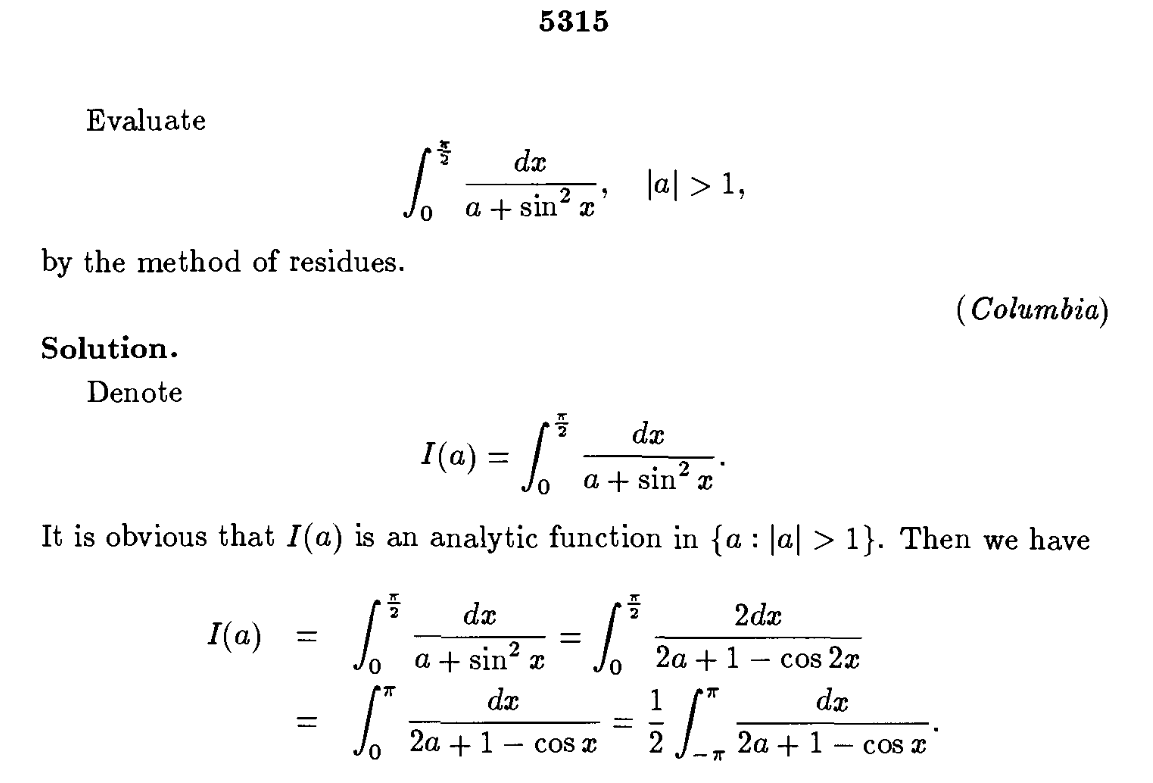
\includegraphics[width=\textwidth]{3-留数计算方法-2025061111.png}
% \caption{}
\label{}
\end{figure}
\begin{figure}[H]
\centering
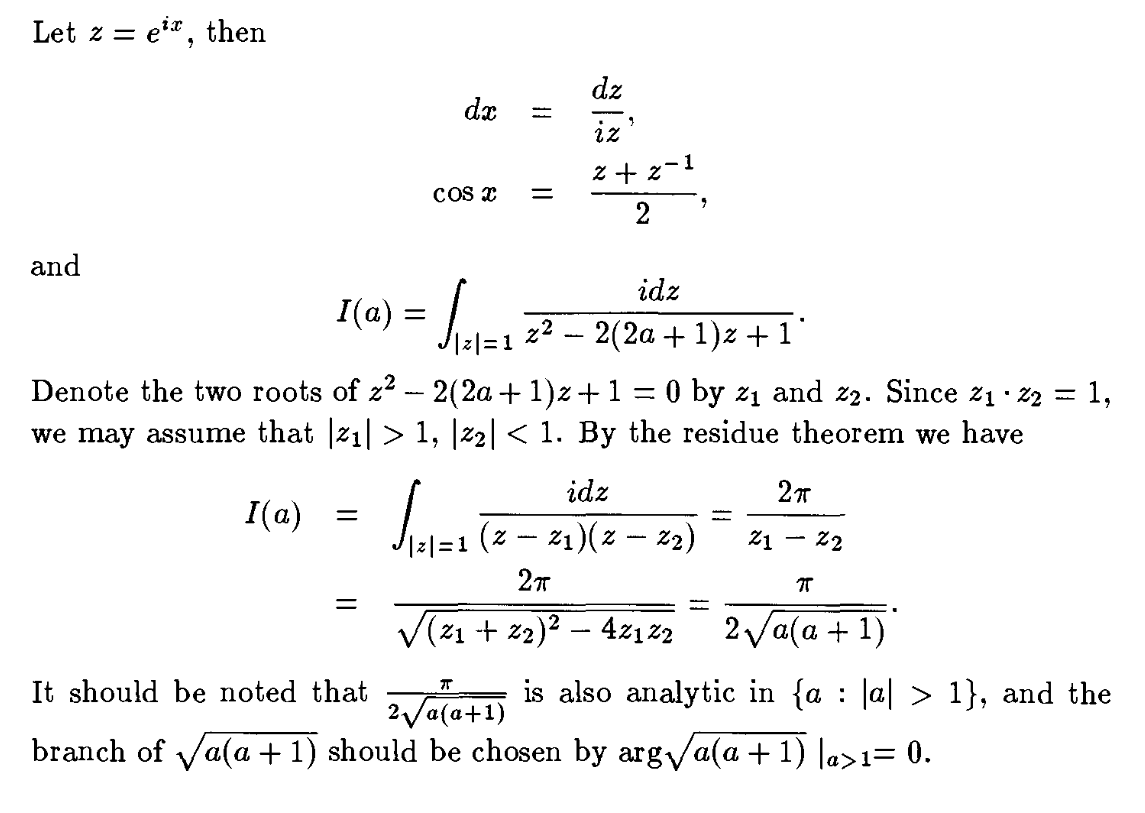
\includegraphics[width=\textwidth]{4-留数计算方法-2025061111.png}
% \caption{}
\label{}
\end{figure}

\subsection{有关 \texorpdfstring{$\log z$}{log z} 的积分恒等式}

\begin{figure}[H]
\centering
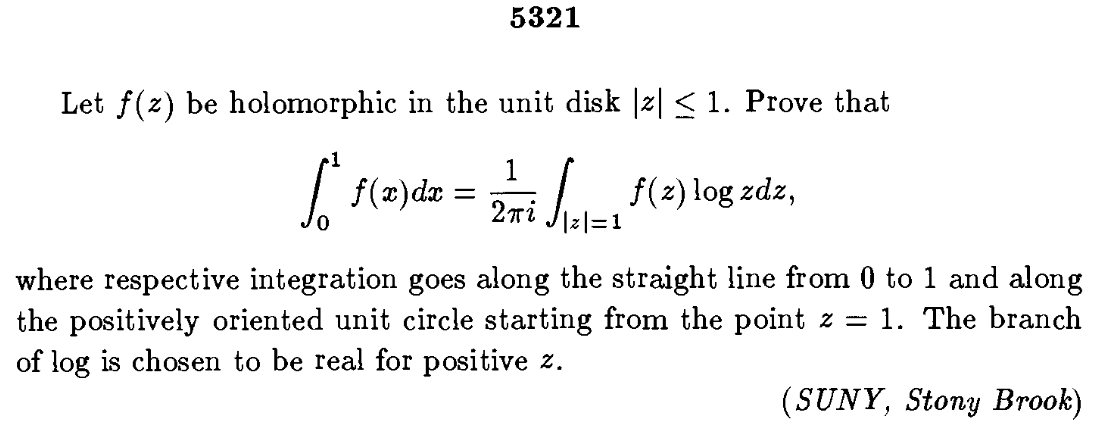
\includegraphics[width=\textwidth]{5-留数计算方法-2025061111.png}
% \caption{}
\label{}
\end{figure}
\begin{figure}[H]
\centering
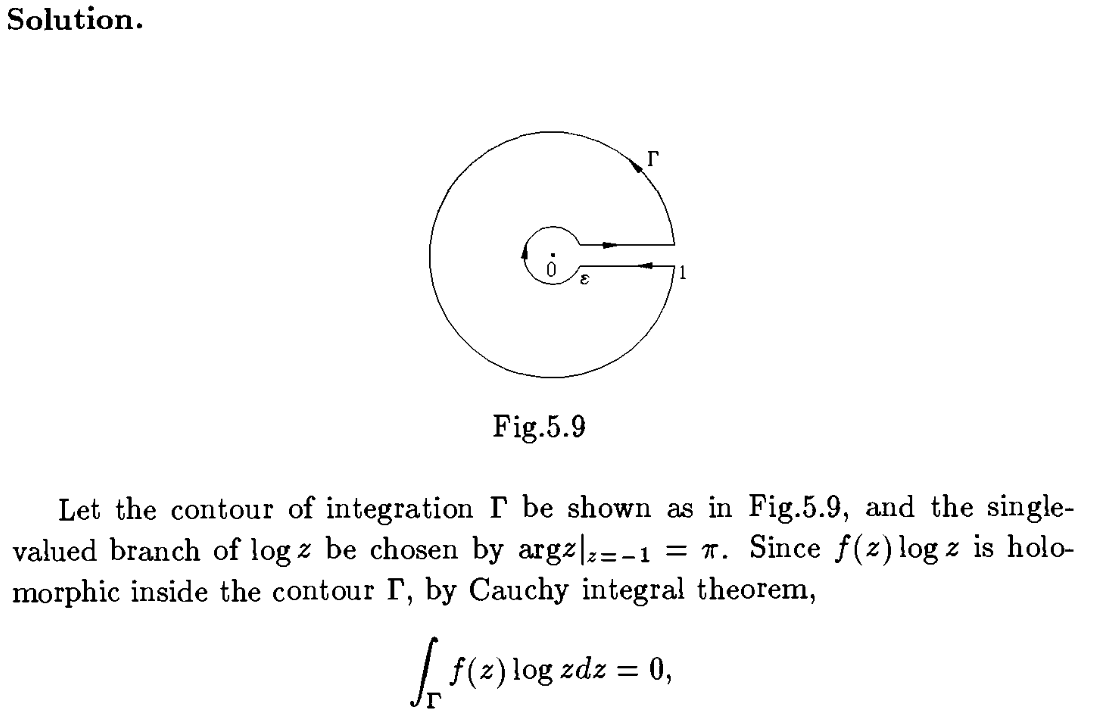
\includegraphics[width=\textwidth]{6-留数计算方法-2025061111.png}
% \caption{}
\label{}
\end{figure}
\begin{figure}[H]
\centering
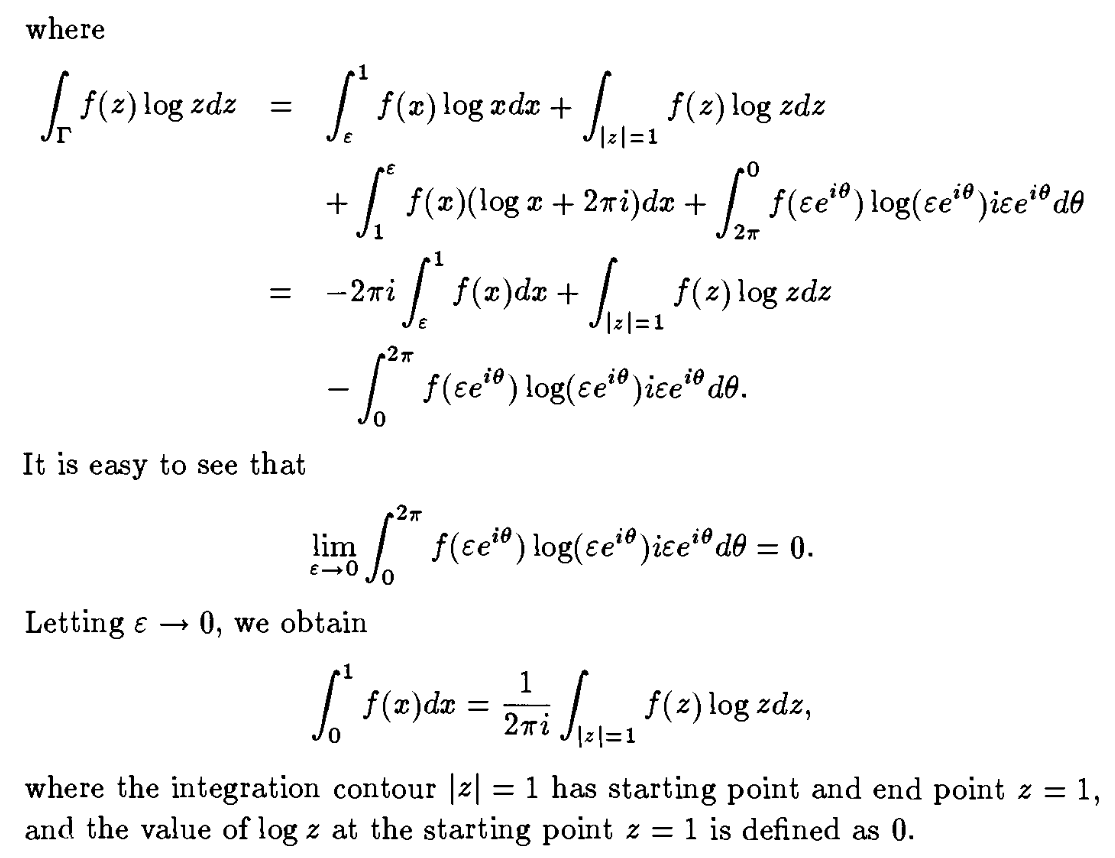
\includegraphics[width=\textwidth]{7-留数计算方法-2025061111.png}
% \caption{}
\label{}
\end{figure}

\subsection{\texorpdfstring{$\log \lvert a+be^{ i\theta } \rvert$}{log lvert a+be^ itheta  rvert} 的积分}

\begin{figure}[H]
\centering
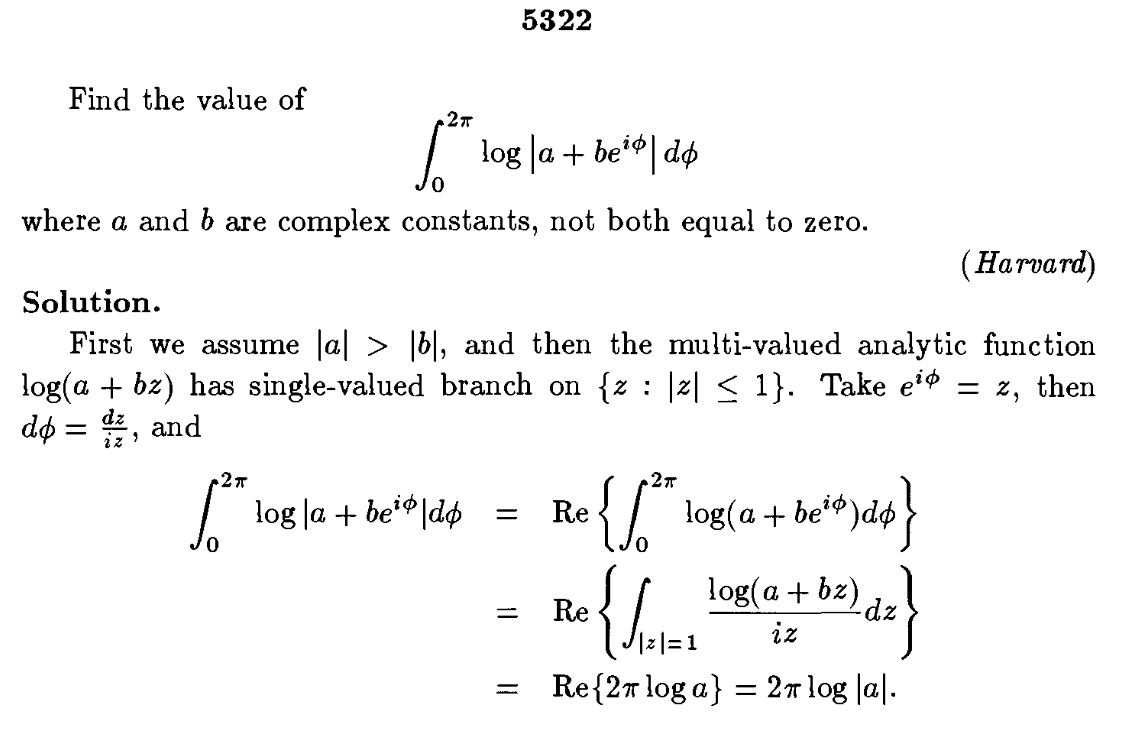
\includegraphics[width=\textwidth]{8-留数计算方法-2025061111.png}
% \caption{}
\label{}
\end{figure}
\begin{figure}[H]
\centering
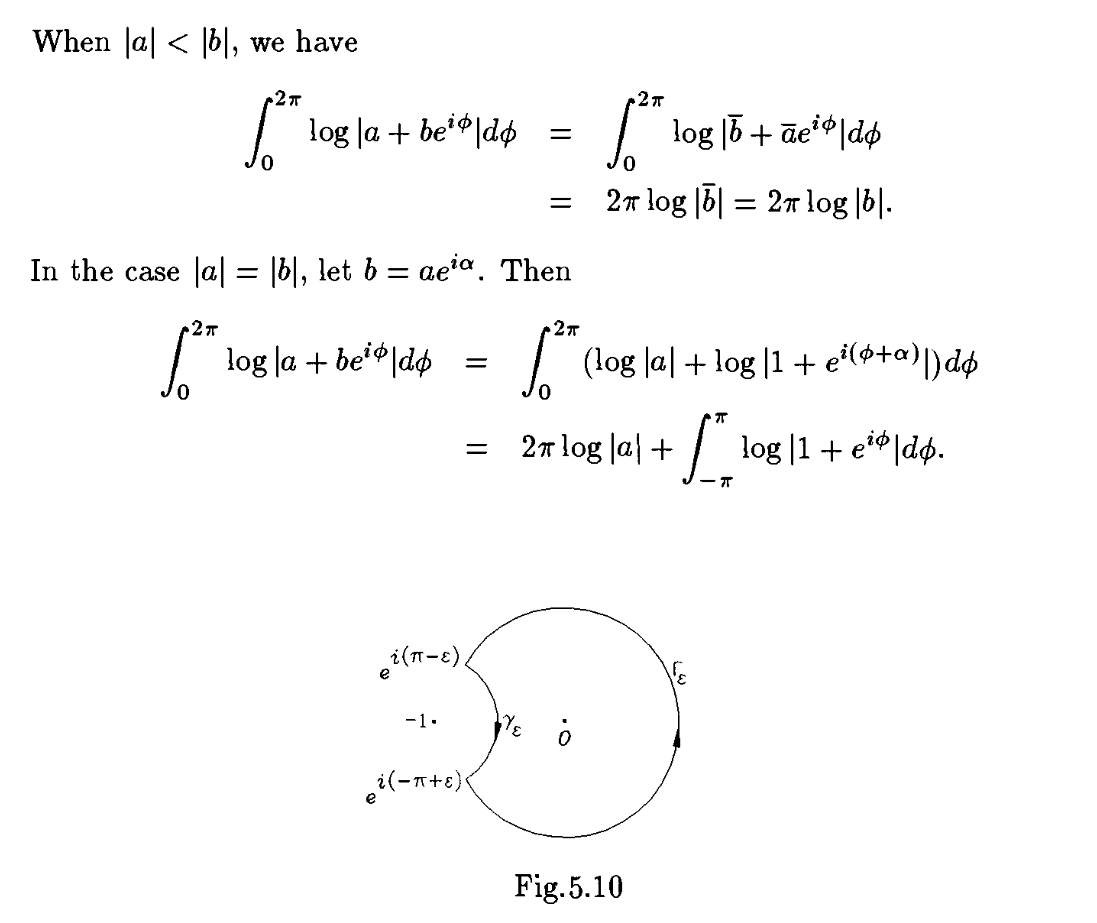
\includegraphics[width=\textwidth]{9-留数计算方法-2025061111.png}
% \caption{}
\label{}
\end{figure}
\begin{figure}[H]
\centering
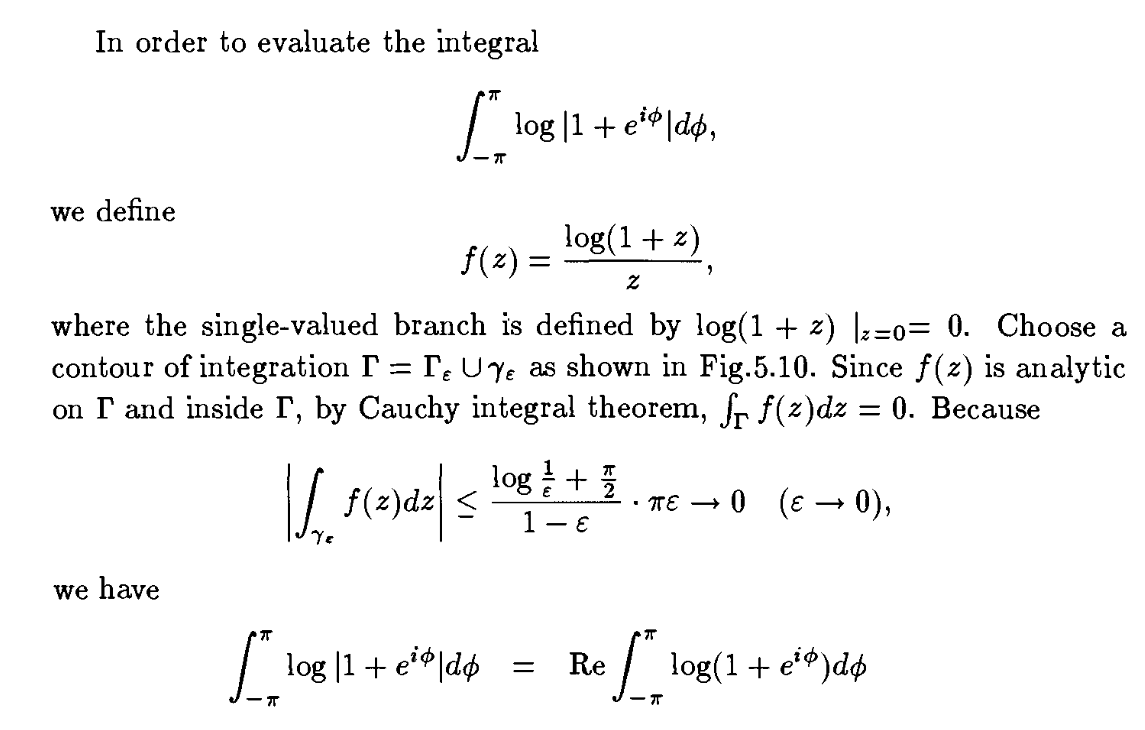
\includegraphics[width=\textwidth]{10-留数计算方法-2025061111.png}
% \caption{}
\label{}
\end{figure}
\begin{figure}[H]
\centering
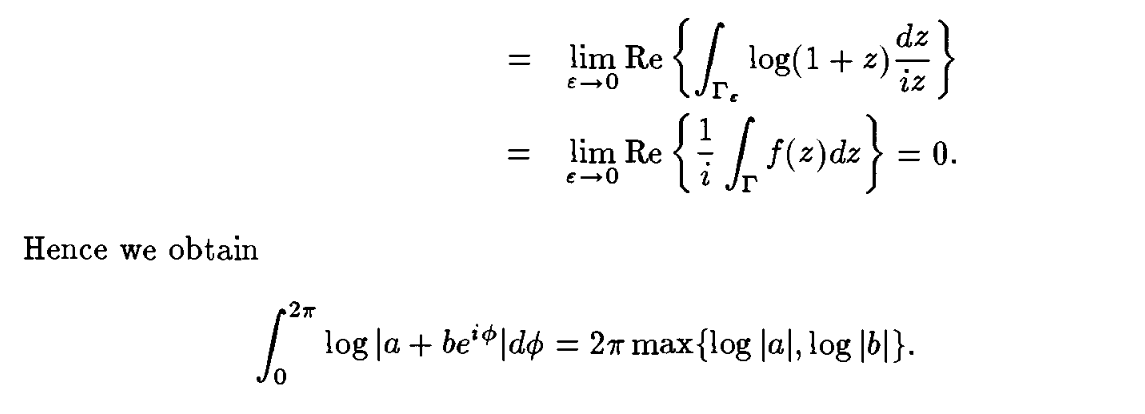
\includegraphics[width=\textwidth]{11-留数计算方法-2025061111.png}
% \caption{}
\label{}
\end{figure}

\subsection{带有 \texorpdfstring{$\log x$}{log x} 的积分,考虑辅助函数带有 \texorpdfstring{$\log ^{2}z$}{log ^2z}}

\begin{figure}[H]
\centering
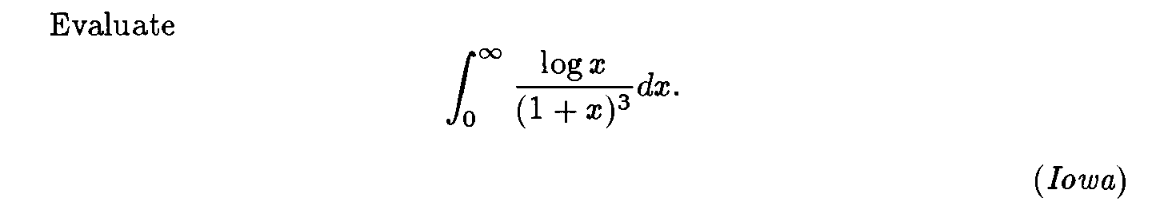
\includegraphics[width=\textwidth]{12-留数计算方法-2025061111.png}
% \caption{}
\label{}
\end{figure}
\begin{figure}[H]
\centering
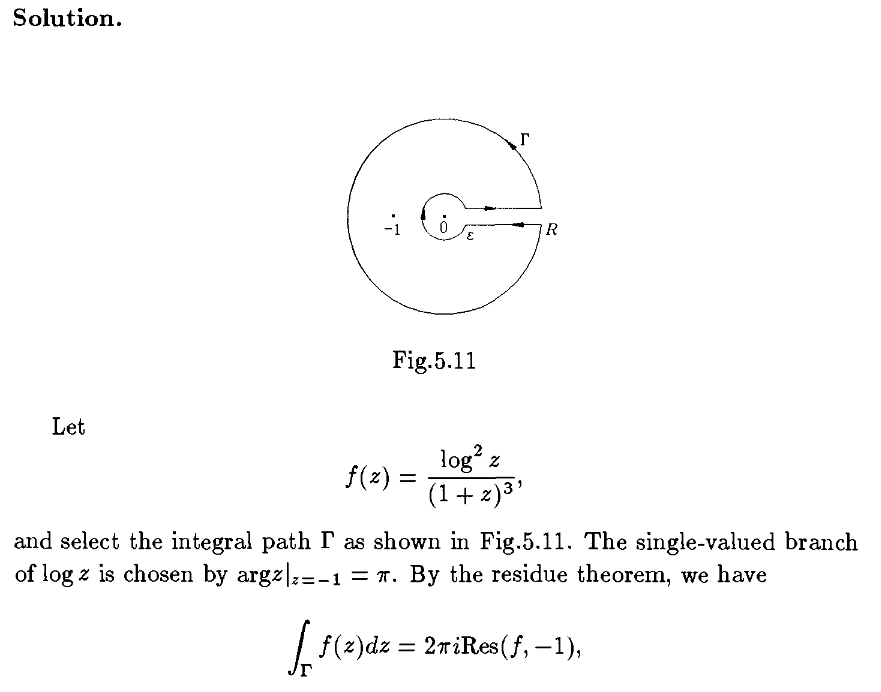
\includegraphics[width=\textwidth]{13-留数计算方法-2025061111.png}
% \caption{}
\label{}
\end{figure}
\begin{figure}[H]
\centering
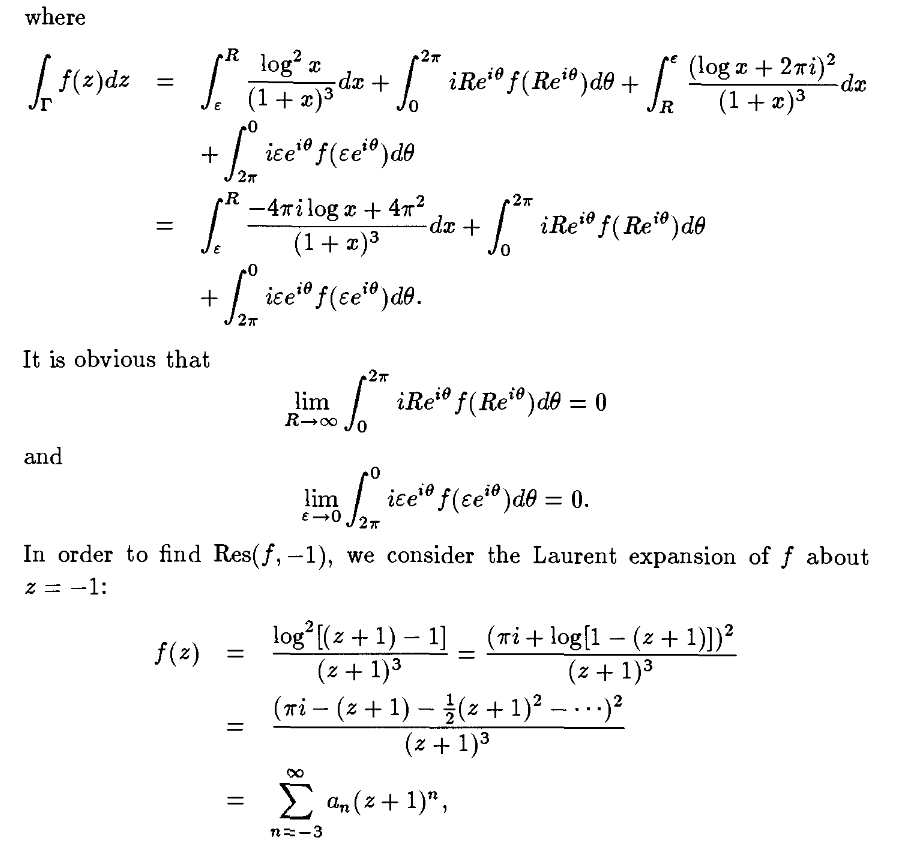
\includegraphics[width=\textwidth]{14-留数计算方法-2025061111.png}
% \caption{}
\label{}
\end{figure}
\begin{figure}[H]
\centering
\includegraphics[width=\textwidth]{15-留数计算方法-2025061111.png}
% \caption{}
\label{}
\end{figure}
